%!TeX root = ../main.tex
\chapter{Quantification of perfusion exams: A~review}\label{chapter:review}

Generally speaking, quantification of perfusion consists in deriving parameters from blood flow measurements, regardless of the method used for the measure. 
This topic has been on the table, and continuously evolving, long before perfusion imaging existed. 
Indeed, G.N.~Stewart introduced indicator dilution theory, starting with the founding paper published in the Journal of Physiology in 1897~\cite{Stewart:1897dz}. 
Indicator dilution theory was originally developed to quantify perfusion using blood sampling data.
It relates tracer concentration curves to physical measurements, i.e.~blood flow, blood volume, and mean transit time, assuming a stationary flow system and an instantaneous injection of a known quantity of tracer.
W.F.~Hamilton went further, corrected some approximations made by Stewart.
Even before Stewart and Hamilton, hemodynamics of the heart had been studied  through indirect measurements and reported in German language by \citet{Volkmann:1850us} and \citet{Vierordt:82xUDMVI} in the 1850s, and later through direct measurements by \citet{Stolnikow:1886wm} and \citet{Tigerstedt:1891wn}.

This chapter fundamentally aims to review the various methods used to quantify perfusion exams acquired using one of the imaging modality briefly presented in Chapter~\ref{chapter:intro}. 
Quantification of perfusion exams is possible assuming the signal intensity is linearly related to the concentration of tracer in the tissue. 
Verifying this assumption is not included in the scope of this thesis, it will therefore be considered true in the following of this manuscript.
Additionally, perfusion imaging modalities yields macroscopic measurements, i.e.~at the pixel or voxel level, and does not give direct access to microscopic measurements, i.e.~at the cellular or molecular level.
Therefore, an image-based measurement is really a mixture of multiple signals corresponding to the various vascular structures present inside the unitary volume of interest. 

Realistically, this review of perfusion quantification techniques cannot be close to comprehensive, instead it tackles the subject from the three angles mentioned thereafter, and emphasis the major landmarks of the perfusion quantification landscape.
Section~\ref{sec:SQMethods} presents semi-quantitative methods, extracting parameters directly either from raw or noise-filtered enhancement curves. 
Then Section~\ref{sec:DeconvolutionMethods} presents deconvolution-based quantification methods, estimating the impulse response in the tissue of interest by means of blind or regularized deconvolution.
Finally, compartmental models accounting for the various interactions of the contrast agent with the tissue are presented in Section~\ref{sec:CompartmentalModels}. 

\section{Semi-quantitative methods}
\label{sec:SQMethods}
\subsection{Generalities}
Semi-quantitative methods are probably among the most intuitive as they extract perfusion-related parameters directly from raw, interpolated, or noise-filtered enhancement curves.
They are however not directly related to any physiological function and are prone to changes in experimental or physiological conditions.
They are therefore often used as relative indicators of perfusion and contrast agent transit time~\cite{Miles:1991et}, allowing intra-exam comparisons.

Examples of semi-quantitative parameters include the peak enhancement~\cite{Norman:1978ji,Nally:1985te,Pettersson:1987ft,Erlemann:1989ib}, the time to peak enhancement~\cite{Norman:1978ji,Erlemann:1989ib,Dietrich:2012kw}, maximum upslope gradient, also known as wash-in rate~\cite{Nally:1985te,Erlemann:1989ib}, the area under the enhancement curve~\cite{Dietrich:2012kw}. 
We also considered semi-quantitative the perfusion parameters based on indicator dilution theory that were derived from the previously cited parameters~\cite{Hilson:1978us,Peters:1987fa,Peters:1987vx,Miles:1991et,Miles:1991ei,Miles:1993cq,Blomley:1995vs,Koenig:1998ir}.
Figure~\ref{fig:SQParameters} shows graphical representations of the above mentioned semi-quantitative parameters. 

\begin{figure}[ht]
  	\centering
  	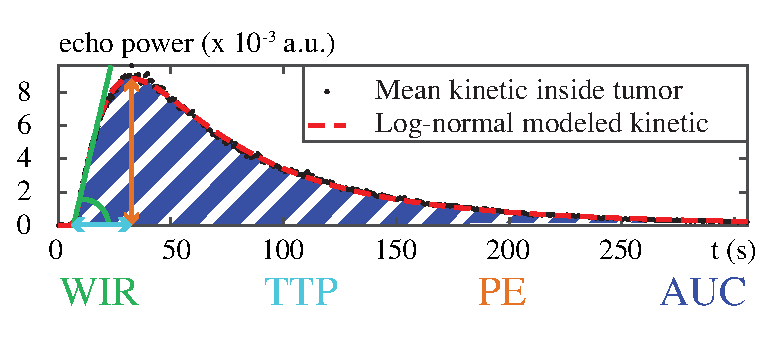
\includegraphics[width=0.6\textwidth]{SQParameters.eps}
	\caption{Examples of semi-quantitative parameters are illustrated on the mean kinetics (black dots) inside the perfused area of a murine tumor observed in contrast-enhanced ultrasound and fitted with a log-normal model (red dashed line): the wash-in rate ($WIR$, in green), the time-to-peak ($TTP$, in cyan), the peak enhancement ($PE$, in orange), and the area under the curve ($AUC$, in dark blue).} 
  	\label{fig:SQParameters}
\end{figure}

\subsection{Nuclear medicine}
\label{sec:SQNM}
Semi-quantitative parameters have been used to differentiate stenosed from healthy kidney in scintigraphy exams, i.e.~a nuclear medicine technique using a gamma camera, following bolus injection of $\left[^{99m}Tc\right]$DTPA.

For instance, \citet{Hilson:1978us}~and later \citet{Peters:1987fa}~both proposed an enhancement-based perfusion index, which is commonly defined as the ratio of the tissue blood flow to the cardiac output. 
On the one hand, \citet{Hilson:1978us}~defined the perfusion index as the ratio of the area under the arterial curve to the area under the renal curve, both curves are integrated up to the arterial peak.
On the other hand, Peter et al.~defined the perfusion index as the ratio of the maximum upslope of the renal curve normalized for the injected quantity to the maximum upslope of the integrated arterial curve normalized for the area under the arterial enhancement curve, and multiplied by a constant converting the number of received gamma photons into a unit of activity~\cite{Peters:1987fa,Peters:1987vx}. 

\citet{Nally:1985te}~reported significant differences in the wash-in rate, curve width at 75\% of the peak enhancement, and maximum enhancement in normal and stenosed kidney in a canine model. 


\subsection{X-ray imaging}
\label{sec:SQRadiography}
Derived from the work of \citet{Peters:1987fa}, semi-quantitative parameters were also proposed by Miles et al.~in \citeyear{Miles:1991et} to quantify renal cortical and medullary perfusion in X-ray computed tomography (CT) with bolus injection of Iodine~\cite{Miles:1991et,Miles:1991ei}. 
The proposed perfusion index was defined as the ratio of the maximum slope in the tissue curve and the peak enhancement of the arterial curve. 
The method was successively used to quantify perfusion in the pancreas~\cite{Miles:2014ea}, solitary pulmonary nodules~\cite{Zhang:1997bi}, lymphoma masses~\cite{Dugdale:1999co}, lung adenocarcinoma~\cite{Tateishi:2001fz}, and more generally to study tumor angiogenesis~\cite{Tateishi:2001fz,Miles:2002eu}.

Miles et al.~also adapted the method to account for both arterial and venous perfusion of the liver, using the splenic enhancement as venous input because the portal vein was not present in the image~\cite{Miles:1993cq}.
Arterial perfusion was calculated using the maximum slope before peak splenic enhancement, while venous perfusion was calculated using the maximum slope after peak splenic enhancement.

In 1995 Blomley et al.~proposed the liver subtraction method to quantify liver perfusion~\cite{Blomley:1995vs}. 
Instead of estimating the upslope in the late liver enhancement curve, they first subtracted the splenic enhancement curve multiplied by the ratio of arterial to splenic arterial perfusion, i.e. the ratio of the maximum slope in the early liver enhancement curve to the maximum slope in the spleen. 
The maximum slope of the corrected enhancement curve is then used to calculate portal perfusion.
In this study, the time and value of peak enhancement were obtained using a gamma variate fit, allowing a finer estimation of these parameters.
Whenever possible the authors used the enhancement curve in the portal vein instead of the splenic vein.
Authors demonstrated the use of portal perfusion in one patient with metastatic livers, as well as in four patients with cirrhotic livers.
Facing the small number of cases in the previous study, a collaborating group extended the application of the method in cirrhotic livers with more cases~\cite{Tsushima:1999vc}.
They estimated arterial and portal perfusion in a group of twenty patients with viral-induced cirrhosis and in fourteen controls. 
While arterial perfusion did not differ between groups, they found a significant reduction in portal perfusion among patients compared to controls, and a strong correlation between portal perfusion and the prothrombin ratio which is an indicator of hepatic parenchymal damage.

Inspired by the work of Miles et al., the method was adapted by Koenig et al.~in \citeyear{Koenig:1998ir} to quantify perfusion in the brain in order to detect and assess cerebral ischemia in acute stroke~\cite{Koenig:1998ir}. 
While arterial enhancement could be estimated from small vessels present in the image, it was not used due to peak attenuation by partial volume effects. 
Instead, the peak venous enhancement in the superior sagittal sinus was used. 
The authors reported relatively small approximation error, with slightly flattened enhancement curves, explained by the short transit time of the contrast agent in brain tissues.
The cerebral blood flow, commonly noted CBF, is the equivalent of the perfusion index in brain tissues. 
The authors defined it as the ratio of the maximum slope of the tissue enhancement curve to the peak enhancement in the superior sagittal sinus.
The fractional cerebral blood volume, commonly noted CBV, was defined as the ratio of the peak tissue enhancement to the peak enhancement in the superior sagittal sinus. 
In a following study~\cite{Klotz:1999ef}, the authors assess the linearity, the spatial resolution, and the sensitivity to noise of CBF through simulations and phantom study, and investigated the relative CBF estimated using large hemispherically mirrored regions of interest using follow-up CT and MR data. 
They reported a systematic underestimation of CBF correlated with the cardiac output of the patient, a good linearity of relative CBF, and recommend using the relative parameter as a predictor of the reversibility of an ischemic stroke.


\subsection{Magnetic resonance imaging}
\label{sec:SQMR}
Following the methodological developments of Gadolinium-DTPA complex (Gd-DTPA) by \citet{Weinmann:1984gv,Brasch:1984cz}, and \citet{Wesbey:1984is} in \citeyear{Weinmann:1984gv} supported by qualitative visual analysis, various applications of the technique emerged in the field of oncology.

Quantification attempts started with the work of \citet{Felix:1985fv} in 1985 using Gd-DTPA enhanced images acquired 5 minutes after injection of the contrast agent. 
Results were compared with pre-contrast MR images obtained using various acquisition sequences and X-ray CT imaging with injection of a iodinated contrast agent. 
They obtained accurate contours of brain tumor and necrosis with no significant enhancement in the region exhibiting peritumoral edema.
They also attempted to differentiate the various types of tumor included in their study based on the contrast index before and after injection of Gd-DTPA. 
The index is defined as the ratio of signal intensity in the tumor tissue to the signal intensity in normal brain tissue. 
It is the first semi-quantitative parameter used for Gd-DTPA enhanced MRI. % Felix:1985fv

\citet{Revel:1986ix} assessed the difference in signal intensity between the pre-contrast and 25-minute post-contrast images acquired in the largest section of subcutaneous human breast tumors implanted in mice.
Signal intensity in the tissue were normalized by the signal intensity in a corn-oil phantom visible in every image. 
Limited by the temporal resolution of their acquisition, authors do not comment on the temporal evolution of signal intensity, despite intermediate acquisitions performed respectively 5 and 15 minutes after Gd-DTPA injection. % Revel:1986ix

\citet{Pettersson:1987ft} performed repeated acquisitions of multiple MR sequences in rabbits subcutaneously implanted with a Vx2 tumor model, and additional induced hemorrhage in surrounding muscle tissue. 
Temporal evolution of enhancement is assessed more finely than in previous studies, acquiring an image every 2.5 minutes for the first 10 minutes after injection of Gd-DTPA and then every 5 minutes for the following 20 minutes.
This allowed the authors to observe that no substantial enhancement occurred in abnormal tissues after 10 minutes, however they only reported on variations of peak signal intensity. % Pettersson:1987ft

In \citeyear{Erlemann:1989ib}, \citet{Erlemann:1989ib} investigated dynamic contrast-enhanced MRI using a T1-weighted spin-echo sequence every 20 seconds following bolus injection of Gd-DTPA as a tool to differentiate tumors from healthy tissue in musculoskeletal lesions.
Their primary result was an increase in contrast-to-noise ratio between tumor and muscle compared to T2-weighted images, and a decrease in contrast-to-noise ratio between tumor and bone marrow or fatty tissue compared to non-enhanced T1-weighted images. 
Additionally, they estimated the baseline signal intensity, the maximum signal intensity, and the time-lapse between the start of the injection and the point of maximum signal intensity. 
Using these estimates, the defined the signal intensity ratio as the percentage of increase over the baseline signal intensity, as well as the relative enhancement slope.
They observed an increase of the signal intensity ratios and relative enhancement slope in malignant tumors compared to benign tumors, the latter showing smaller overlap between malignant and benign groups.
Enhancement slope enabled malignancy prediction with an accuracy of 79.7\% using a cutoff value of 30\%/min.
They also reported lower peak intensity ratios and wash-in rates in areas with necrosis or peritumoral edema. % Erlemann:1989ib

% Wilke:1993wu, Contrast-enhanced first pass myocardial perfusion imaging: correlation between myocardial blood flow in dogs at rest and during hyperemia.
\citet{Wilke:1993wu} investigated the use of contrast-enhanced magnetic-resonance imaging for the quantification of myocardial perfusion in a canine study, and compared the estimated parameters to the blood flow obtained using radiolabelled microspheres.
A bolus of Gd-DTPA was injected during Turbo-FLASH acquisition, and a six circular regions of interest were delineated in the myocardium, as well as one region of interest in each ventricular cavity, yielding a total of nine regional time-intensity curves.
All the time-intensity curves were fitted with a gamma-variate curve to both correct for recirculation, and limit the impact of extravascular diffusion, using only the samples occurring before the curves decreases to 70\% of its peak value.
The mean transit time of each curve was calculated numerically, and the correlation of its inverse, of the time of peak intensity, as well as the initial slope (defined as the ratio of the peak intensity to the time of peak intensity) with absolute myocardial blood flow estimates from radiolabelled microspheres were investigated.
Good correlations with the ground truth ($r \geq 0.89$) were reported for the three semi-quantitative parameters cited above.

\citet{Verstraete:1994iw} also reported on the ability to differentiate benign from malignant musculoskeletal lesions, using imaging and quantification techniques similar to those used by \citet{Erlemann:1989ib}.
Despite the higher temporal resolution of 2.41 seconds possible in their study, their findings are likewise nuanced because of the overlap of parameters between highly vascularized benign lesions and the malignant ones. % Verstraete:1994iw

\citet{Baur:1997ur} reported higher signal intensity ratios after injection of Gd-DTPA in patients with intermediate-grade and high-grade diffuse malignant bone marrow infiltration in the spine compared to healthy patients.
Nonetheless, they were unable to detect low-grade lesions using this technique, and reported large variabilities in all patient groups. % Baur1997

\subsection{Ultrasound}
\label{sec:SQCEUS}
The current section addresses the semi-quantitative methods used to quantify perfusion using ultrasound.
Refer to Section~\ref{sec:IntroCEUS} for more information on contrast-enhanced ultrasound as a perfusion imaging modality, including the nature of the contrast-agent, the image formation processes, as well as the various injection techniques.
Methods assessing perfusion using bolus injection are first presented, followed by methods specific to continuous infusion injection.

As a foreword to this section, indicator dilution theory as first formalized by \citet{Stewart:1897dz} and later by \citet{Hamilton:1932ww} is valid under the condition that the mass of contrast-agent is conserved through the time of the acquisition. 
Since \citeyear{Butler:1979wu}, it is known that a portion of the intravenously injected microbubbles are filtrated through the lungs~\cite{Butler:1979wu,Meltzer:1980js}
% Butler:1979wu, Journal of Applied Physiology, The lung as a filter for microbubbles
% Meltzer:1980js, WHY DO THE LUNGS CLEAR ULTRASONIC CONTRAST?
, i.e.~before their first pass in the tissue of interest.
Moreover, a portion of the following passes is filtered by the Kupffer cells in the liver~\cite{Kindberg:2003iq,Yanagisawa:2007bu}.
% Kindberg:2003iq, Hepatic clearance of Sonazoid perfluorobutane microbubbles by Kupffer cells does not reduce the ability of liver to phagocytose or degrade albumin microspheres
% Yanagisawa:2007bu, PHAGOCYTOSIS  OF  ULTRASOUND  CONTRAST  AGENT MICROBUBBLES  BY  KUPFFER CELLS
Additionally, \citet{Lampaskis:2010fj} % Lampaskis:2010fj, Investigation of the the relationship of nonlinear backscattered ultrasound intensity with microbubble concentration at low MI. 
confirmed that imaging using a high mechanical index disrupts a non-negligible number of microbubbles, and demonstrated that most of the microbubbles disrupted during imaging at a low mechanical-index are actually naturally disrupted. 
The mass conservation condition is therefore usually not respected in contrast-enhanced ultrasound, even in first-pass studies.
Semi-quantitative methods based on indicator dilution theory were nonetheless extensively used to quantify perfusion in contrast-enhanced ultrasound exams.

\subsubsection{Bolus injection}
\label{SQ:US:Bolus}

\paragraph{\em{Model-free quantification methods}\\}

From an historical standpoint, \citet{Bommer:1978eu} were the first to report indicator-dilution curves using contrast-enhanced ultrasound data in an abstract published in The American Journal of Cardiology in \citeyear{Bommer:1978eu}. % Bommer:1978eu, Indicator-dilution curves obtained by photometric analysis of two-dimension echo-contrast studies
Authors used a photometer to quantify the evolution of signal intensity, as visualized on the screen of the monitor.
The enhancement resulted from the venous injection of a bolus of microbubbles, obtained by microcavitations through rapid injection of dextrose in water. 
The indicator-dilution curves were quantified in terms of time from peak enhancement to 50\% decay, and to 90\% decay. 
The latter was found correlated to the cardiac-output, and enabled the differentiation of patients with low and normal cardiac index. 
In the same issue of The American Journal of Cardiology, the same group applied the same technique to produce indicator-dilution curves in another cardiac study~\cite{DeMaria:1978il}. % DeMaria:1978il, Combined peripheral venous injection and cross-sectional echocardiography in the evaluation of cardiac disease
They used the ultrasound images themselves to identify patients with intracardiac shunts, but also the mean clearance time of the indicator-dilution curves to identify patients with tricuspid regurgitation, and severe congestive failure.

At the same period, \citet{Hagler:1982hs} presented early data of videodensitometry data for the quantification of left-to-right shunts using echographic acquisitions with direct injection of a bolus of ultrasound contrast-agent (i.e.~indocyanine green dye) in the left ventricle. % Hagler:1982hs, Videodensitometric Quantitation of Left-to-Right Shunts with Contrast Echocardiography
They estimated the ratio of left-to-right shunt, which they defined as the ratio of the area under the curve in the right ventricle to the area under the curve in the left ventricle, and showed an strong correlation of echographic measurements with both indicator-dilution and dye measurements.
\citet{Meltzer:1982vt} extended this work and investigated the relevance of a mono-exponential model to fit the wash-out curve, as suggested by indicator-dilution theory. % Meltzer:1982vt, Videodensitometric processing of contrast two-dimensional echocardiographic data.
This was assessed by fitting a linear model to the log-transformed time-density wash-out curve, exhibiting excellent correlation with experimental data. 
They therefore concluded on the relevance of the log wash-out slope, and established its relation to the contrast agent disappearance rate. 

Following the early work of \citet{Armstrong:1982tq} and \citet{Tei:1983ul}, \citet{TenCate:1984hl} investigated the use of contrast-enhanced echography for the assessment of myocardial perfusion following intracoronary injection of a bolus injection of microbubbles in a canine study with varying coronary artery flow (using a hydraulic occluder) to simulate ischemia, and with injection of Dipyridamole to dilate the coronary bed and therefore simulate hyperemia.
% Armstrong:1982tq, Assessment of myocardial perfusion abnormalities with contrast-enhanced two-dimensional echocardiography.
% Tei:1983ul, Myocardial contrast echocardiography: a reproducible technique of myocardial opacification for identifying regional perfusion deficits.
% TenCate:1984hl, Myocardial contrast two-dimensional echocardiography: experimental examination at different coronary flow levels.
The microbubbles in this study were investigated in a previous study of the same group, ensuring they were small enough to circulate through capillaries without getting trapped~\cite{Feinstein:1984gk}. 
% Feinstein:1984gk, Two-Dimensional Contrast Echocardiography. I. In Vitro Development and Quantitative Analysis of Echo Contrast Agents
Semi-quantitative functional parameters were extracted from log-compressed time-intensity curves, i.e.~the half wash-in time, half wash-out time (ignoring the recirculation by fitting a mono-exponential model), peak intensity time and value, and total curve duration.
They found significant changes in total curve duration, and in half wash-in and wash-out times, for both ischemia and hyperemia in comparison with control measurements.
Interobserver and intraobserver variability, as well as injection reproducibility was assessed for the half wash-out time, with respective correlation coefficients of 0.98, 0.86, and 0.78.
In addition, the relative systolic wall thickening was also estimated, and while it correlated well with the coronary artery flow measured by an electromagnetic flowmeter placed directly on the artery, no correlation was foud with the ultrasound half wash-out time. 

A few years later, \citet{Vandenberg:1989bza} performed a similar canine study with induced ischemia and hyperemia, intending to predict myocardial blood flow from semi-quantitative parameters derived from contrast-enhanced ultrasound time-intensity curves. 
% Vandenberg:1989bza, Quantitation of myocardial perfusion by contrast echocardiography: Analysis of contrast gray level appearance variables and intracyclic variability
In addition to peak intensity time and value, they investigated the use of the wash-in rate. 
Peak intensity value and wash-in rate were found correlated to myocardial blood flow, however correlations were moderate ($r = 0.67$ and $0.51$ respectively).
However, the relative changes of the wash-in rate exhibited a stronger correlation ($r = 0.77$) with the relative changes of the myocardial blood flow, i.e.~with induced ischemia and hyperemia.

In a clinical study, \citet{TenCate:1987vw} estimated the total curve duration, the area under the curve, and the half wash-out time from time-intensity curves obtained in the ventricular septum from end-diastolic images.
% TenCate:1987vw, Quantitative assessment of myocardial blood flow by contrast two-dimensional echocardiography: initial clinical observations.
They performed multiple regression analysis between the parameters extracted from contrast-enhanced ultrasound data to angiographic parameters, i.e.~the percentage of coronary area stenosis, and the minimal lumen area, derived from data acquired using the protocol described in~\cite{Wijns:1985wz}.
% Wijns:1985wz, Quantitative angiography of the left anterior descending coronary artery: correlations with pressure gradient and results of exercise thallium scintigraphy
Authors reported relations of various natures between the above-mentioned parameters, i.e.~linear, inverse, exponential, and logarithmic.
In particular, the strongest correlation was found between the area under the curve and the percentage of coronary area stenosis (exponential relation). 
Additionally, while all correlation were found significant, this couple of parameters was the only one with a strong correlation ($r \geq 0.8$). 
Noting the discrepancies between the pre-clinical and the clinical results, the authors suggest they found their sources in modifications of the experimental setup, i.e.~the injection method or the nature of the ultrasound contrast agent.

In \citeyear{Bleeker:1990uy}, \citet{Bleeker:1990uy} evaluated the stability, size, and ultrasonic properties of multiple ultrasond contrast agents, and investigated the feasibility of blood flow estimation through in vitro experiments.
% Bleeker:1990uy, On the application of ultrasonic contrast agents for blood flowmetry and assessment of cardiac perfusion.
Their findings were in favor of the Albunex contrast agent, which were the only microbubbles exhibiting sufficiently longlasting stability (i.e.~in size and number) when exposed to ultrasound waves.
In addition, a linear relation between the concentration of microbubbles and both backscatter coefficient (i.e.~reflected power) and attenuation coefficient (i.e.~transmitted power) was reported for low concentrations.
They also found strong linear relations between the ultrasonic properties of the contrast agent and the flow estimated using an indicator-dilution theory.  
They emphasis the questionability of using grey-levels from ultrasound images to characterize blood flow, and instead recommend using attenuation based on transmission techniques, or backscattering after proper correction of signal attenuation.
In vitro experiments showed strong relations between the ultrasonic properties of Albunex contrast agent and the flow estimated using indicator-dilution theory.

A somehow similar in vitro study was conducted a few years later by \citet{Heidenreich:1993ji}, however the proposed quantification model makes use of an input function as a reference instead of the injected quantity used by \citet{Bleeker:1990uy}, and extends the indicator-dilution model to estimate the tissue blood volume and mean transit time, in addition to the tissue blood flow. 
% Heidenreich:1993ji, In vitro calculation of flow by use of contrast ultrasonography.
The model is based on the estimation of the area under the curve and mean transit time for both input and studied tissues.
The ratio of the area under the curve in the studied tissue to the input yields the tissue blood volume, the system mean transit time is approximated as twice the difference in mean transit times, and the tissue blood flow was classically defined as the ratio of tissue blood volume to system mean transit time.
In vitro calibration data revealed the log-compressed nature of the data in the experimental system, allowing linearization of the video intensity for low to moderate concentrations, and therefore conversion to volumetric concentration of microbubbles.
Excellent agreement was found between measured and estimated flow rates, using 39 measurements at low concentration.
Authors report on the difficulty to find a pure blood pool in the ultrasound imaging plane, but also to image both tissue and input with sufficient sensitivity and without saturation artifacts respectively because of the limited dynamic range of commercial ultrasound scanners.
Additionally they comment on the simplicity of the model which allows to alleviate the signal attenuation artifacts which are often non-negligible in-vivo, and on the impossibility to ensure conservation of the contrast agent quantity and properties throughout the acquisition. 

\citet{Aronson:1993wsa}, from the same research group, later assessed the model described above in-vivo, in an attempt to quantify kidney perfusion in a canine study. 
% Aronson:1993wsa, Assessment of renal blood flow with contrast ultrasonography.
A total of 58 bolus injections of microbubbles with varying concentrations (23 for aortic measurements, and 35 for cortical measurements), and 93 bolus injections with modulated blood flow (57 reduction, 10 increase, and 26 controls), were performed in 9 dogs.
Blood flow was controled by means of a renal artery occluder for flow reduction, and dopamine or fenoldopam infusion for flow increase. 
A major limitation of this study lies in the fact that renal and aortic data did not originate from the same injection, as a different dose of contrast-agents was used to extract the time-intensity curves in the two regions of interest.
Additionally, the injected doses were ajusted empirically in order to obtain complete opacification of the region of interest, without reaching the signal saturation threshold.
Direct measurements of blood flow were performed using an electromagnetic flowmeter, for comparison with the value estimated using contrast-enhanced ultrasound.
The major findings of this study are the evidence of a strong correlation between the injected concentration and the pixel intensity, for both cortical and aortic measurements, and strong correlation of the estimated blood flow with in-situ flow measurements with a tendency to overestimate blood flow. 
Authors discuss the various pitfalls of contrast-enhanced ultrasound that could influence the accuracy of the method, including possible changes in blood volume in the modulated flow experiments, signal attenuation, and electronic thresholding.
They finally conclude on the inability to perform absolute quantification of blood flow with the existing apparatus, stating that the major requirements lie in increased linearity and dynamic range.

\citet{Schwarz:1993wp} investigated the use of the wash-out rate from log-transformed time-intensity curves following bolus injection, as well as the ratio of the wash-out rates from two bolus injections with varying flow rates. 
% Schwarz:1993wp, Volumetric arterial flow quantification using echo contrast. An in vitro comparison of three ultrasonic intensity methods: radio frequency, video and Doppler.
Time-intensity curves were obtained using various backscatter intensity techniques, i.e.~radio frequency, video intensity, pulsed wave Doppler, and intravascular Doppler.
Authors obtained strong correlations of the wash-out rate with the in vitro flow rate, however they reported different slopes in two chambers with varying mixing volume.
The relative wash-out rate not only exhibited excellent correlations with the relative flow rate, it also yielded a good agreement of the slopes obtained in the two mixing chambers.
These results suggest the independence of the relative wash-out rate to the mixing volume, and the ability of this parameter to accurately characterize changes in blood flow.

\citet{Wiencek:1993hr} investigated the various steps necessary to achieve accurate quantification of contrast echocardiography using indicator-dilution theory. 
% Wiencek:1993hr, Pitfalls in Quantitative Contrast Echocardiography: The Steps to Quantitation of Perfusion
The proposed approach assumes the arterial input function is known beforehand, i.e.~the time-intensity curve in a pure blood pool like the aortic root or in the left ventricle, in order to relax the need for standardized injection and physiological conditions.
Authors ackowledge the difficulty of estimating the input function using a single injection, and suggest performing two separate injections to avoid saturation and non-linearities caused by high contrast-agent concentrations.
They emphasis the necessity for a consistent and confined range of microbubble size, as the intensity of the signal backscattered by a single bubble is non-linearly proportional to the diameter of the bubble.
The importance of conservation of contrast-agent quantity and properties throughout the acquisition of the ultrasound images was outlined, and the impact of hydrostatic pressure and gas saturation level of the solution as reported in the litterature was investigated.
The choice of the representation of the time-intensity curves, i.e.~video intensity, log-transformed intensity, or concentration from calibration data, and its impact on the estimated parameters were discussed.
A possible explanation for undetected changes when using the peak intensity as an indicator of blood flow was proposed, authors related it to signal saturation and illustrate this phenomenon in simple cases where the changes in blood flow are caused by a change in blood volume only or in transit time only.
Additionally, electronic issues resulting from signal acquisition, signal processing, and electronic thresholding were discussed.
Physiological factors like tissue-dependant hematocrit were also investigated.
Finally, methods which showed promising results in preliminary studies at the time of the review (i.e.~\citeyear{Wiencek:1993hr}) were reported, including various alternative imaging schemes (e.g.~acoustic velocity, radiofrequency data, second harmonic imaging).

\paragraph{\em{Model-based quantification methods}\\}

% Kaul:1989il, Assessment of regional myocardial blood flow with myocardial contrast two-dimensional echocardiography
In \citeyear{Kaul:1989il}, \citet{Kaul:1989il} proposed a first-order gamma variate model to quantify blood flow using consecutive contrast-enhanced echocardiography acquisitions in an open-chest canine study with varying blood flow. 
They compared their results in the myocardium and in the coronary bed with the transmural myocardial blood flow measured using radiolabelled microspheres, and to direct coronary flow measurements obtained by an electromagnetic flowmeter. 
They studied the influence of the injection site by performing their experiments in two groups of eight dogs. 
In the first group, dogs were injected a bolus of microbubbles in the circumflex artery, while in the second group they were injected in the left main coronary.
Authors reported a good correlation of both myocardial and coronary blood flow measurements with the parameter of the gamma variate model which influences the width of the modeled enhancement curve, $\alpha$, for both groups (mean $r = 0.81$ and $0.96$ respectively), but a poor correlation of the peak intensity (mean $r = 0.63$ and $0.39$ respectively). 
Pooling estimates from the eight dogs did not affect the correlation with $\alpha$ for the first group ($r = 0.80$), however for the second group, pooling data considerably dropped the correlation ($r = 0.23$).
Scattered plots reveal the varying slopes obtained in the different dogs, emphasizing the impact of the injection site.
Indeed, when injecting in the left main coronary the contrast agent is dispersed through the coronary tree, making quantification of myocardial blood flow intrinsically relative.
Authors suggested that absolute quantification of myocardial blood flow may be possible, injecting closer to the branches of the coronary tree, but were well aware that the proposed semi-quantitative parameters are not absolute themselves.

\citet{Tiemann:2000wl} investigated the ability of harmonic power Doppler imaging to yield quantitative perfusion parameters, as this modality inherently destroys microbubble to produce contrast-specific images~\cite{Tiemann:1997vj}, through in vitro experiments, and ex vivo experiments in a porcine heart.
% Tiemann:2000wl, Are microbubbles free flowing tracers through the Myocardium? Comparison of indicator-dilution curves obtained from dye dilution and echo contrast using harmonic power Doppler imaging.
% Tiemann:1997vj, Stimulated Acoustic Emission Nonbackscatter Contrast Effect of Microbubbles Seen with Harmonic Power Doppler Imaging.
They compared the time-intensity curves obtained from harmonic power Doppler, and the time-concentration curves of ICG measured with an extravascular densitometer, to direct flow measurements from a calibrated ultrasonic flowmeter. 
Authors fitted a log-normal model to the experimental curves, since this model has been commonly used to fit indicator-dilution curves~\cite{Stow:1954ty,Wise:1966ji},
% Stow:1954ty, An empirical formula for indicator-dilution curves as obtained in human beings
% Wise:1966ji, The geometry of log-normal and related distributions and an application to tracer-dilution curves
and was later applied in cardiology studies~\cite{Linton:1995ij,Band:1997ib}.
% Linton:1995ij, A new method of analyzing indicator dilution curves
% Band:1997ib, The shape of indicator dilution curves used for cardiac output measurement in man
The area under the curve and the mean transit time of the fitted model were estimated for both modalities. 
While the area under the curve expectedly correlated with the injected quantity of ultrasound contrast agent, the inverse of the mean transit time obtained using microbubbles and ICG measurements exhibited very strong correlation to the direct flow measurements in both in vitro and ex vivo setups.
% Fisher2002, Myocardial and microcirculatory kinetics of BR14, a novel third-generation intravenous ultrasound contrast agent.
% Lagged-normal model for CEUS, estimation of relative peak intensity
However, the mean transit time obtained with harmonic power Doppler time concentration curves was slightly lower than with ICG densitometry, especially for high flow rates.
While most studies used electromagnetic flowmeters as ground truth, this one used an ultrasonic transit-time flowmeter. 
The presence of ultrasonic microbubbles could therefore influence the ground truth flow measurement, and possibly affect the correlation between ultrasonic measurements, however measurements were in agreement with densitometric ICG measurements which alleviates the suspicion.

% Postert:2000kda, Contrast agent specific imaging modes for the ultrasonic assessment of parenchymal cerebral echo contrast enhancement.
In \citeyear{Postert:2000kda}, \citet{Postert:2000kda} proposed an empirical model for the quantification of cerebral perfusion time-intensity curves following intravenous injection of a bolus of microbbubles, imaged through the acoustic temporal bone window using phase-inversion harmonic ultrasound imaging, contrast burst imaging, and time variance imaging for comparison. 
The model accounts for the baseline-intensity and for the maximum intensity variation, i.e.~the peak-intensity minus the baseline-intensity. 
Moreover, the wash-in of the bolus is modeled by a logistic curve with adjustable steepness and delay, despite authors describe it as step function, and the destruction of microbubbles is modeled by an exponential decay.
However, none of the model parameters is directly related to the physiology or to physical measurements. 
Authors used the peak-intensity, as well as the time to peak-intensity extracted parameters from the modeled time-intensity curves as semi-quantitative parameters to compare the values obtained using the three modalities of contrast-enhanced ultrasond cited above, and in four regions of interest of nine healthy patients. 
The study concludes by stating the higher sensitivity of contrast burst imaging and time variance imaging compared to phase-inversion harmonic imaging.

% Eyding:2003bo, Parameters of cerebral perfusion in phase-inversion harmonic imaging (PIHI) ultrasound examinations.
However, three years later, a study by \citet{Eyding:2003bo} to which Postert collaborated, investigated the 90\% peak width as an additional parameters to characterize time-intensity curves from phase-inversion harmonic imaging fitted with this model.
Semi-quantitative parameters were evaluated in five regions of interest of the established ipsilateral view, i.e.~imaging only the hemisphere on the probe side, using an imaging depth of 100 mm, and nine regions of interest using the novel bilateral view, i.e.~allowing simultaneous imaging of both hemishperes with a single probe, using an imaging depth of 150 mm, of fourteen healthy patients. 
Consecutive transtemporal acquisitions following intravenous injection of two different ultrasound contrast agents were performed in each view of each patient, with twenty minute intervals, with for comparison purposes.
The authors reported the sensitivity of peak-intensity to depth, and the ability to differentiate arteries using either time parameter.

% Krogias:2005hs, Semiquantitative analysis of ultrasonic cerebral perfusion imaging.
In a following study~\cite{Krogias:2005hs}, the same group performed another transtemporal contrast-enhanced ultrasound study using the bilateral approach with a single bolus injection in twenty healthy patients.
A total of fourteen regions of interest was delineated in both hemishperes, yielding as many time-intensity curves, from which were estimated the same three semi-quantitative parameters after fitting the empirical model described above. 
Peak intensity was once again excluded from further analysis because of the strong variations among patients.
Because of the small amount of corresponding regions in the study, only descriptive data is presented in the form of aligned boxplots, as if all patients exhibited the same median value. 
The authors recommended the use of the time parameters, in particular the time to peak intensity, as estimated with the bilateral protocol.
They believe it could be a relevant indicator to help characterize lesions in patients with acute strokes, provided that one of the hemispheres is unaffected and can be used as a reference.

% Elie2014, Method and system for quantification of tumoral vascularization (US PATENT: US 8847960 B2)
% IGR custom model
In 2006, \citet{Elie2014} filed a patent application for quantification approach developed specifically for contrast-enhanced ultrasound.
The formulation of the mathematical medel is empirical, and is inspired from the model first proposed by \citet{Eyding:2003bo}, replacing both the numerator and the denominator terms by sigmoid functions. 
A dozen of semi-quantitative parameters that can be derived from the fitted model for vascularization and tumoral angiogenesis detection are listed by the authors, i.e.~peak time, peak value, wash-in time, mean transit time, area under the curve, wash-in rate, area under the wash-in, and under the wash-out. 

% Lavisse:2008gc, Early quantitative evaluation of a tumor vasculature disruptive agent AVE8062 using dynamic contrast-enhanced ultrasonography.
The group later used the patented model in an early attempt to assess the efficacy of a disruptive anti-angiogenic treatment~\cite{Lavisse:2008gc}.
They assessed tumor vasculature through the peak time and peak value, as well as the full-width at half maximum, in four groups of ten mice, respectively imaged at 5, 15 minutes, one hour, six hours, and twenty-four hours after treatment injection, and compared the post-treatment contrast-enhanced ultrasound results to pre-treatment results.
Results were also compared to power Doppler and histology findings.
They reported a progressive decrease in peak-intensity value reaching its minimum six hours after injection of the anti-angiogenic treatement, and opposite effects in time to peak-intensity and in the full-width at half maximum.

% Mischi:2003ed, Videodensitometric Methods for Cardiac Output Measurements
In \citeyear{Mischi:2003ed}, \citet{Mischi:2003ed} proposed the local density random walk model for characterization of tissue perfusion in contrast-enhanced ultrasound with bolus injection of microbubbles. 
The model, first proposed by \citet{Sheppard:1951we} characterizes the dilution process through a mono-dimensional approximation of the vascular network, i.e.~vessels are considered as straight tubes with constant flows, and a Brownian motion of the contrast-agent following bolus injection is assumed.
A novel estimation method based on a two-phase multiple linear regression is proposed, aleviating the need for initialization and assumptions on the nature of the time-intensity curve.
They also proposed a correction for the systematic negative estimation bias in the area under the curve, that was shown proportional to the noise level through simulations.
From the fitted time-intensity curve, the area under the curve and the mean transit time are extracted.
Then flow and volume parameters are derived using the injected quantity of contrast-agent and indicator-dilution theory.
They tested their model in vitro, and compared the flow estimated with contrast-enhanced ultrasound with the direct flow measurements of an electromagnetic flowmeter.
The fitted curves were strongly correlated to the experimental data ($r^2 \gt 0.95$), and so were the four estimated and measured flow values ($r^2 \gt 0.99$).

% Mischi:2004cn, Contrast echocardiography for pulmonary blood volume quantification
In \citeyear{Mischi:2004cn}, \citet{Mischi:2004cn} presented a method to quantify blood volume using the flow and mean transit time estimated in two time-intensity curves derived from contrast-enhanced ultrasound bolus acquisitions, i.e.~respectively acquired upstream and downstream of the volume of interest.
The expression of blood volume is derived from indicator-dilution theory, and is expressed as the product of the difference in mean transit times with the blood flow.
The local density random walk model and the first passage time model were fitted to time-intensity curves to estimate the mean transit time and the flow, and the blood volumes and mean transit times estimated using the two models were then compared through both in vitro and in vivo clinical experiments.
These two models were described by \citet{Walley:1964fr} and \citet{Wise:1966wy}, the main difference between them being that the second only accounts for the first passage of the indicator through the sampling site.
They were compared by \citet{Bogaard:1986wp} in conductivity and thermodilution curves, but this comparison had never been performed for time-intensity curves derived from contrast-enhanced ultrasound data.
Note that the flow was estimated as the ratio of the injected dose to the area under the fitted curve following to indicator-dilution equations presented by Stewart~\cite{Stewart:1897dz} and Hamilton~\cite{Hamilton:1932ww}.
The authors reported a good agreement between the true and estimated values obtained in the in vitro experiments despite some discrepancies, especially for high blood volumes, and a good agreement between the two models for the clinical data in the absence of ground truth.

% Mischi:2008fe, On the physical and stochastic representation of an indicator dilution curve as a gamma variate
% Physical and stochastic explanation of the gamma variate model, comparison with LDRW
In \citeyear{Mischi:2008fe}, \citet{Mischi:2008fe} established the relation of the commonly-used gamma variate model to indicator-dilution theory using a one-dimensional multi-compartmental approximation of the vascular network.
They first gave a physical interpretation, that consists in defining a blood vessel as a cascade of equal mixing chambers, each compartment having a constant flow, and an exponential impulse response with a time constant equal to the ratio of the compartment blood flow to the compartment blood volume.
They also gave a stochastic intrepretation, that models the dilution impulse response at a given distance from the injection site, assuming a Poisson distribution of the number of individual particle wash-out to the next compartment.
Then they revealed the inverse relation between the parameters of the two interpretations, yielding an expression of the tissue impulse response as a function of the wash-out rate and the mean transit time which respects indicator-dilution theorems in the case of an ideal Dirac injection.
They finally established the relation of the gamma variate model with the local density random walk model using the previously presented physical interpretation.
Based on the previously presented methodology~\cite{Mischi:2004cn}, the authors were able to estimate the volume of dilution between two measurements of the same bolus, i.e.~before and after the passage of the bolus in the volume to be estimated.
They performed in vitro experiments with bolus injection, and compared the ability of the two models to estimate the dilution volume in a varying flow setup.
Their in vitro findings were compared to those obtained in vivo, through a cardiac clinical study including twenty patients.
Time-intensity curves in the left and right ventricle of the heart were derived from contrast-enhanced ultrasound acquisitions following bolus injection of microbubbles in an antecubital vein, using the same imaging apparatus and injection protocol than in vitro.
They reported that both models were able to accurately fit both in vitro and in vivo time-intensity curves, and reported on the sensitivity of the local density random walk to initialization.
In vitro, the volume estimations were almost perfectly correlated to the real values using either model, and in good agreement in terms of absolute values, despite the underestimation in the largest volume case.
In vivo, because no ground truth was available, they reported on the differences in the estimates of the two models against the mean estimated value through a Bland-Altman plot, and showed a mean difference of 63.1 mL with a standard deviation of 69.7 mL, representing 11.1\% of the overall mean estimated volume.

% Kuenen:2011kr, Contrast-Ultrasound Diffusion Imaging for Localization of Prostate Cancer
In \citeyear{Kuenen:2011kr}, \citet{Kuenen:2011kr} proposed a modified local density random walk model to reveal diffusion instead of perfusion, motivated by the assumption that this process better reflects tumor angiogenesis. 
They observed that one of the parameters of the local density random walk model is related to the diffusion coefficient, but that it cannot be interpreted locally in-vivo because of its dependance on the distance from the injection site. 
They therefore proposed the replacement of the global boundary condition assuming a Dirac bolus injection, which time and distance are needed, by a local boundary condition assuming a normally distributed spatial concentration profile at the time immediately preceding the passage of the bolus at the sampling location.
Replacing the old global boundary condition by the new local one yields a new expression of the local density random walk model, from which a local diffusion-related parameter $\kappa$ can be derived, defined as the ratio of the diffusive time to the squared convective time.
The accuracy of the method was investigated by fitting the model to synthetic time-intensity curves simulated using the convective diffusion equation. 
The model was able to fit the simulated curves accurately, and $\kappa$ was estimated with a mean relative error of 4\%. 
However, when considering curves with recirculation and therefore fitting the model on cropped curves, the authors reported a higher mean relative error of 10\%. 
Clinical relevance of the method was assessed in a preliminary study including five datasets from four patients with confirmed prostate cancer, that were referred for radical ablation of the prostate. 
Parametric maps of $\kappa$ were compared to histology-based tissue classification, i.e.~based on the level of cell differenciation.
In all patients, authors were able to discriminate cancerous from healthy tissue, i.e.~cancerous regions were associated with high $\kappa$ values.
The tissue classification power of both classical semi-quantitative parameters and the parameters of the proposed model was investigated. 
Optimal threshold values used for classification were estimated through histogram analysis.
The authors acknowledge that the proposed diffusion-related parameter, $\kappa$, was not the most sensitive investigated parameter, however it was the only one with both sensitivity and specificity above 80\%.
It also exhibited the highest area under the receiver operating characteristic curve with a value of 0.909. 

% Averkiou:2010iw, Quantification of Tumor Microvascularity with Respiratory Gated Contrast Enhanced Ultrasound for Monitoring Therapy.
In an attempt to monitor the microvascularity of colorectal metastasis in the liver of patients undergoing anti-cancer treatment, \citet{Averkiou:2010iw} investigated the use of the ratio of the wash-in time in the metastasis to the wash-in time in normal liver parenchyma.
They proposed an empirical model based on the error function to estimate the wash-in time of respiratory-gated time-intensity curves in metastatic and normal tissues obtained by contrast-enhanced ultrasonography.
The function under investigation is a time-delayed error function, member of the sigmoid family, with varying rise time and maximum intensity, fitted to the wash-in of the time-intensity curve.
Authors stated the rise time parameter is linearly related to the wash-in time.
They performed a reproducibility study in five untreated patients with a total of twelve acquisitions, with varying injected quantity and/or injection duration of contrast-agent from one acquisition to another.
While the wash-in time in the metastatic tissue exhibited variations up to 30\%, the wash-in time ratio was more reproducible exhibiting an average deviation of 9\%, with a maximum of 16\%, revealing the effect of normalization.
The ability of the wash-in time ratio to assess treatment efficiency was investigated in a longitudinal study, performed in seven patients undergoing a combination of cytotoxic and antiangiogenic treatments.
Major findings include the ability to discriminate good from bad responders to therapy, the ground truth responder classification being assessed by experts using conventional criteria, i.e.~number and size of the lesions, blood tests for serum tumor markers, and liver function tests.
Indeed, four out of five good responders exhibited a significant rise of the wash-in time ratio after the first therapy cycle, revealing the early normalization of the lesion microvascularity, and the mean increase in wash-in time ratio among the good responders at the end of the treatment was 75\%.

\subsubsection{Infusion injection}
In 1998, \citet{Wei:1998jd} proposed an explicit model to quantify myocardial perfusion. % Wei:1998jd, Quantification of myocardial blood flow with ultrasound-induced destruction of microbubbles administered as a constant venous infusion
For this method, microbubbles were injected as a continuous infusion.
When the micro-bubble concentration reached a steady state, high mechanical index ultrasound pulses were used to disrupt microbubbles in the myocardium with increasing pulsing interval.
This technique is known as intermittent imaging.
The video intensity, which was assumed proportional to the concentration in microbubbles, was plotted as a function of the pulsing interval. 
Then an exponential function with plateau value $A$ and rate constant $\beta$ was fitted. 
Assuming a constant beam elevation, \citet{Wei:1998jd} demonstrated that blood flow $F$ was proportional to the slope at the origin, i.e.~$A\beta$.
The authors validated their approach in vitro, but also ex vivo and in vivo in a canine study.
The method was later validated for perfusion quantification of the kidney, estimating both cortical and medullary blood flow in another canine study~\cite{Wei:2001id}. % Wei:2001id, Quantification of renal blood flow with contrast-enhanced ultrasound

The development of power pulse inversion imaging by \citet{Simpson:1997jn} in \citeyear{Simpson:1997jn}, % Simpson:1997jn, Pulse inversion Doppler: A new method for detecting nonlinear echoes from microbubble contrast agents
allowing real-time imaging of low microbubble concentration at low mechanical index~\cite{Tiemann:1999vy}. % Tiemann:1999vy, Real-time contrast echo assessment of myocardial perfusion at low emission power: First experimental and clinical results using power pulse inversion imaging
\citet{Tiemann:1999vy} in \citeyear{Tiemann:1999vy} % Tiemann:1999vy, Real-Time Contrast Echo Assessment of Myocardial Perfusion at Low Emission Power: First Experimental and Clinical Results Using Power Pulse Inversion Imaging.
and \citet{Masugata:2001vg} in \citeyear{Masugata:2001vg} % Masugata:2001vg, Quantitative Assessment of Myocardial Perfusion During Graded Coronary Stenosis by Real-Time Myocardial Contrast Echo Refilling Curves
demonstrated the use of power pulse inversion to image the replenishment of tissue following a single series of microbubble-disrupting pulses in real-time.
Both studies also reveal that the model proposed by \citet{Wei:1998jd} could be used to accurately fit real-time replenishment curves.

In \citeyear{Schlosser:2001vv}, \citet{Schlosser:2001vv} applied the same model to quantify renal perfusion, % Schlosser:2001vv, Feasibility of the flash-replenishment concept in renal tissue: which parameters affect the assessment of the contrast replenishment?
and compared the estimated parameters according to the acquisition sequence, i.e.~power pulse inversion~\cite{Simpson:1997jn} vs.~pulse inversion~\cite{Burns:2000tl}. % Burns:2000tl, Pulse inversion imaging of liver blood flow: improved method for characterizing focal masses with microbubble contrast
The authors disclosed highly different perfusion parameter values according to the acquisition scheme, which yielded significantly different values of both parameters.
However, they were able to distinguish large arteries in the renal hilum from smaller arteries in the renal cortex, using either of the schemes, and either of the parameters.

% Krix2003tq, A multivessel model describing replenishment kinetics of ultrasound contrast agent for quantification of tissue perfusion
In \citeyear{Krix:2003tq}, ~\citet{Krix:2003tq} presented a hyperbolic model to quantify perfusion using either intermittent or real-time imaging, relying on physiological considerations, and accounting for the distribution of blood velocities in the tissue.  
The model assumes a spherical distribution of blood vessel directions with varying blood velocity.
This assumption yields an initial linear increase of the concentration until the vessels perpendicular to the imaging plane with the highest velocity are fully refilled. 
After the initial linear increase in signal intensity, the fully filled vessels do not contribute to signal increase anymore. This yields a non-linear increase until only the vessels with the lowest velocity remain to be fully filled. 
Finally, all the vessels present in the imaging plane are fully filled and a plateau intensity is reached. 
Authors describe an iterative method to estimate the instant of maximum and mean velocity.
They state the slope of the replenishment curve observed at these times can be used to evaluate the maximum blood velocity in the region of interest, assuming the width of the ultrasound beam is known.
The influence on the width of the blood velocity distribution is visually described.
The method was evaluated in a murine study with continuous infusion and intermittent imaging, followed by a bolus injection and intermittent imaging as well~\cite{Krix:2003wh}. % Comparison of intermittent-bolus contrast imaging with conventional power Doppler sonography: quantification of tumour perfusion in small animals

% Potdevin:2004eq, Analysis of refill curve shape in ultrasound contrast agent studies
\citet{Potdevin:2004eq} investigated the misfit of the exponential model to refill curves and proposed the use of the error function instead.
They introduced a time-delay parameter in their model in order to better reflect experimental data. 
They also investigated the impact of observing multiple blood velocities in the region of interest, as well as the effect of the point spread function of the imaging system through a simulation study and concluded that replenishment curves contain more information that just mean transit time. 
For instance they were able to reveal the presence of abnormal vascular structures, such as shunting, i.e.~direct flow from the arterial system to the venous system without passing through the capillary bed.
In a latter study, they proposed an adaptation of the model to quantify local replenishment curves in tissues with complex vascular structures.
Replenishment curves are first normalized according to the estimated depth-dependent pixel intensity in a pixel containing only blood.
The model accounts for the specific angles, lengths, and velocities of the various vascular structures in the studied tissue~\cite{Potdevin:2006fs}. % Potdevin:2006fs, Refill model of rabbit kidney vasculature
They also used their model as a tissue classifier tool, determining tissue type as the predefined vascular model that best fitted the enhancement curve in the least squares sense.
However, applying the simpler exponential model with the average tissue mean transit time on normalized data yielded accurate tissue classification maps, suggesting that the major factor differentiating the replenishment curves of the various tissue types is actually mean transit time.
The additional information could be used to characterize vascular properties more finely.
In spite, while their is no physical evidence why the exponential model should fit replenishment curves, it remains a good approximation and allows accurate differentiation among tissue types.
This is especially true when applied to noisy replenishment curves.

\citet{Arditi:2006ip} introduced a new formalism for the quantification of real-time destruction-replenishment acquisitions using a low mechanical index. % Arditi:2006ip, A new formalism for the quantification of tissue perfusion by the destruction-replenishment method in contrast ultrasound imaging 
The authors emphasize the importance of linearizing ultrasound data according to the type and settings of the imaging equipment, as opposed to grey levels intensities directly extracted from the log-compressed images visible on the monitor.
More importantly, they present a perfusion model accounting for the variety in blood flow velocity and direction, assuming a model accurately describing the distribution of transit times is known (e.g.~log-normal distribution).
The method achieves a better description of the S-shaped replenishment curves that can be observed.

In \citeyear{Quaia:2009fs}, \citet{Quaia:2009fs} proposed a model reflecting the drag (related to flow) and diffusion (not related to flow) of microbubbles in blood, and accounting for the variety of blood velocities and directions. % Quaia:2009fs, ASSESSMENT OF A NEW MATHEMATICAL MODEL FOR THE COMPUTATION OF NUMERICAL PARAMETERS RELATED TO RENAL CORTICAL BLOOD FLOW AND FRACTIONAL BLOOD VOLUME BY CONTRAST-ENHANCED ULTRASOUND
This variety is modeled as the sum of a variable number of piecewise linear replenishment curves.
The model was validated through in vitro experiments using a dialysis cartridge with tubular capillaries, and in vivo experiments in the renal cortex of 12 healthy volunteers, separated in two age groups. 
While it achieved a significantly better fit than the exponential model using a Wilcoxon signed-rank test, whether the proposed model was using two, three, or four different tracts, the differences in the mean squared error remained extremely small and exhibited non-negligible overlap.
Furthermore, while the authors report a significant difference in the initial replenishment slope among the two age groups using the proposed model, based a Mann-Whitney U-test, they do not report on the slope differences obtained using the exponential model, nor on the apparent concordance of the plateau values obtained using the two models.

\section{Deconvolution methods}
\label{sec:DeconvolutionMethods}
\subsection{Generalities}
Deconvolution-based methods are model-free approaches, assuming a linear and stationary system without any assumption on the underlying structures and processes~\cite{Lassen:1979tk}.
% Lassen:1979tm, Tracer kinetic methods in medical physiology, Ch9. Convolution Analysis
Resolving the deconvolution equations necessitates the knowledge of at least two measurements: an input function, and either a residual measurement (i.e.~the amount of tracer remaining in the system) or an output measurement (i.e.~the amount of tracer leaving the system).
In particular, dynamic perfusion imaging grants access to spatially-distributed measurements of the residual tissue function.

The resolution process aims at estimating the impulse-response function of the system, which is theoretically independant on the input, and because no assumption is made on the structure of the system, no assumption is made on the shape of the impulse-response function or on the unit of the measurements.
Additionally, the impulse-response function can be seen as the probability distribution of the contrast particles transit times~\cite{Lassen:1979vj}.
% Lassen:1979vj, Tracer kinetic methods in medical physiology, Ch. 7 MTT: Bolus Injection
Parameters describing the systemic response of the vascular system can therefore be derived from the impulse-response function estimated by deconvolution.

% Zierler:1962cx, Theoretical Basis of Indicator-Dilution Methods For Measuring Flow and Volume
In \citeyear{Zierler:1962cx}, \citet{Zierler:1962cx} established the relevance of the impulse response to assess indicator-dilution curves.
He deeply investigated the theoretical aspects of indicator-dilution theory, the conditions for its validity, and the consequences when they are not respected, including when a sudden injection is not truly instantaneous. 
This section established the theoretical basis for deconvolution of indicator-dilution curves. 
In another section addressing the impact of recirculation, he established the role of the Laplace transform when solving convolution integrals, as found in his theoretical framework.

% Coulam:1966un, A transfer function analysis of coronary and renal circulation calculated from upstream and downstream indicator-dilution curves
In \citeyear{Coulam:1966un}, \citet{Coulam:1966un} proposed deconvolution to estimate the impulse response of coronary and renal circulatory systems, as well as the global circulatory impulse response, in a canine study with one dog.
Because a perfect impulse injection is not achievable in practice, the impulse response cannot be estimated directly from the downstream time-concentration curve.
Therefore bolus injections of indocyanine green dye were performed in a pulmonary artery and blood was sampled at various downstream sites.
Deconvolution of the downstream curves by the upstream curve was performed in the frequency domain by simple division of the Fourier coefficients, and the inverse transform was applied to obtain the impulse response in the time domain.
The accuracy of the estimation was assessed both visually and numerically, through time-domain convolution of the estimated impulse response with the upstream curve, yielding an estimate of the downstream curve. 
Using simulations, the role of the number of harmonics present in the upstream curves was investigated.
Indeed, for low numbers of harmonics, oscillations could occur in the impulse response, yielding inaccurate estimation.
The authors suggest intra-ventricular injection would alleviate this issue, as the upstream curve would contain more harmonics.

% Maseri:1970gn, Frequency function of transit times through dog pulmonary circulation
In \citeyear{Maseri:1970gn}, \citet{Maseri:1970gn} used deconvolution to estimate the impulse response of the pulmonary circulatory system.
Two tracers were injected simultaneously, the first one in the pulmonary artery, and the second one in the left ventricle.
Both tracers were sampled at the same site, at the aortic root, yielding two time-concentration curves. 
The authors used Laplace transforms to demonstrate that deconvolving the first time-concentration curve by the second one yields the impulse response of the pulmonary circulatory system, independently of the systemic recirculation of the tracers. 
The deconvolution was performed using numerically without any curve fitting, despite the reported unstability of the solution.
In order to limit this instability, the experiments were adapted consequently. 
Visual checking was used to assess the accuracy of the estimation, and manual correction was performed when necessary.
Biases induced by correction of recirculation through mono-exponential interpolation of the wash-out were reported in case of early recirculation.

% Valentinuzzi:1975tr, Discrete deconvolution
A popular matrix-based deconvolution technique was proposed by \citet{Valentinuzzi:1975tr} in \citeyear{Valentinuzzi:1975tr}. 
The method relies on the matrix formulation of the convolution process, however the set of derived linear equations is solved successively, therefore avoiding matrix inversion which is known to be an ill-conditioned problem. 
Authors acknowledge the sensitivity of the technique to noise, and warn about the impact of imperfect noise filtering on the estimation process. 
The role of the sampling interval is also discussed, the authors reveal that increasing it can only improve estimation accuracy up to a point, but demonstrated that increasing it too much could actually increase the estimation error.

% Knopp:1976uc, Transcoronary intravascular transport functions obtained via a stable deconvolution technique
In \citeyear{Knopp:1976uc}, a deconvolution method said to be insensitive to noise, recirculation, and impulse response shape was proposed by \citet{Knopp:1976uc} to assess the impulse response of the coronary bed.
The method was tested in a canine study with intra-ventricular injection dye injection, and simultaneous blood sampling at the aortic root and in the coronary sinus.
The technique first models the impulse response as a weighted sum of delayed statistical distributions with unit area, which allowed predetermination of the convolved curves and aleviated the signal periodicity condition, and then iteratively minimized the fit error using a gradient descent algorithm.
Impulse functions were first investigated, however other distribution functions were chosen to reduce the computational load while making the estimation more robust and ensuring similar quality of fit.
Experiments reveal right-skewed impulse responses with prolonged tails, suggesting non-monoexponential downslopes expected using classical unimodal functions, i.e.~lagged-normal, gamma-variate, lognormal.
The authors compared their estimates of mean and standard deviation of transit times to the estimates from previous studies, performed by the same group, but focused on other vascular structures, i.e.~lungs~\cite{Knopp:1969tu}, descending aorta~\cite{Bassingthwaighte:1967vy}, and femoral artery~\cite{Bassingthwaighte:1966jn}. 
Despite the reported parametric overlap, authors observed a rise of the relative variation of transit times correlated with the complexity of the vascular structures, which they justified by reminding that different pathways have different mean transit times and flows.

% Gamel:1973uz, Pitfalls in digital computation of the impulse response of vascular beds from indicator-dilution curves
As soon as \citeyear{Gamel:1973uz}, \citet{Gamel:1973uz} published a review of the various pitfalls affecting the deconvolution process when estimating tissue impulse responses from indicator-dilution curves. 
The impact of noise on the estimation of the impulse response by the direct method was first demonstrated on simulated data, establishing the necessity of either using an appropriate noise filtering technique, enforcing some predetermined form to the impulse response, or applying some kind of regularization to the estimation process in order to avoid oscillations and negative values.
Six estimation methods enforcing either of the above mentioned strategies were then investigated regarding various considerations.
The impact of the data starting point was investigated, especially in the output curve which is usually widely spread and delayed.
The authors report poor impulse response estimation in case of noisy time-varying data, despite the accuracy of the reconvolved curves.
Then the impact of the numerical approximation which is a consequence discretization process was investigated, while trapezoidal integration exhibited lower error than rectangular integration, both methods proved extremely sensitive to noise. 

% Lassen:1984kp, Cerebral transit of an intravascular tracer may allow measurement of regional blood volume but not regional blood flow.
Additionally, in \citeyear{Lassen:1984kp} \citet{Lassen:1984kp} warned about the inability to estimate the blood flow unless the shape of the impulse response is accurately known prior to deconvolution.
He said this was necessary in order to accurately determin the height of the initial bolus.
And while this is not the object of his letter, he also warned about the lack of direct relations between blood flow and the various semi-quantitative parameters proposed in the litterature.

\subsection{Nuclear medicine}
% Kenny:1975gl, Deconvolution analysis of the scintillation camera renogram.
Following the development of renography based on gamma-camera acquisitions by \citet{Short:1973ip}, \citet{Kenny:1975gl} used a deconvolution technique first presented in \cite{Fleming:1974id}, based on the Laplace transform, in an attempt to make the estimation of the kidney function independent on the spread of the bolus when it enters the kidney, and assessed it in a clinical study.
% Fleming:1974id, A technique for the deconvolution of the renogram
The approach accounts for both the establishment of an equilibrium of the tracer in the extravascular space, spread of the bolus during its passage through the kidney, and the removal of the tracer from blood by the kidney assuming bi-exponential clearance in the cardiac measurements.
The impulse response of the kidney vascular network was estimated from the Laplace-derived formula established in the paper, involving the renal time-activity curve, its derivative, its integral and various constants to be estimated.
Because scintigraphy is a projection imaging technique, the background activity was subtracted using the regions between the two kidneys to obtain the activity as specific to the kidney as possible.
This was encouraged by the similarity of the activity curves in this region with those of the nephrectomy sites observed in fifteen kidney-ablated subjects.
Authors were able to distinguish healthy kidneys from those affected by various diseases, indeed all affected kidneys exhibited longer minimum, mean, and maximum transit times, and a wider transit time distribution.
Additionally, they were able to distinguish between the various studied diseases using the same criteria.
% Appledorn:1977hl, Deconvolution analysis of the scintillation camera renogram. (response)
\citet{Appledorn:1977hl} responded to the publication and expressed his disagreement regarding the formulation of the clearance function, arguing that the input to the renal system depends on the negative time derivative of the cardiac curve.
He explained his reasoning mathematically, assuming a two-compartment model previously presented in the litterature~\cite{DeGrazia:1974uo}, and proposed a correction for the renal input function. 

% Diffey:1976tk, The 99mTc-DTPA dynamic renal scan with deconvolution analysis.
\citet{Diffey:1976tk} proposed the use of the matrix-based deconvolution method, first generically introduced by \citet{Valentinuzzi:1975tr}, to quantify the impulse responses of the renal parenchyma and renal pelvis to a bolus injection of $^{99m}$Tc-DTPA. 
% Diffey:1976bf, Data-bounding technique in discrete deconvolution
They used the iterative data-bounding technique prior to deconvolution for noise removal, the technique is detailed in~\cite{Diffey:1976bf}.
Non-renal activity is assumed qualitatively similar to arterial activity, thus the correction is simply applied by setting the first term of the impulse response equal to the second one.
The impulse response of the renal parenchyma was obtained by deconvoluting the parenchymal curve by the arterial curve.
The impulse reponse of the renal pelvis was obtained by deconvoluting the pelvic curve by the parenchymal curve.
Accounting for the regional variations of tracer retention enabled the authors to differentiate between patients with and without pelvic obstruction, and proved to be an efficient tool to assess the renal function.
Authors regret that the spatial resolution of the gamma-camera did not enable to distinguish between cortical and medulary structures.

% Alderson:1979ts, Deconvolution analysis in radionucleide quantitation of left-to-right cardiac shunts
In \citeyear{Alderson:1979ts}, a Fourier-based deconvolution technique, relying on the same computational technique as~\cite{Coulam:1966un}, was proposed by \citet{Alderson:1979ts} to quantify left-to-right cardiac shunts from time-activity curves from scintigraphy following bolus injection of $[^{99m}$Tc]pertechnetate in a canine study. 
The shunt quantification technique used the gamma-fitting technique first presented by \citet{Maltz:1973jj}, and was preceded by either low-pass filtering in the frequency domain, or smoothing of the deconvolved curves in the time domain, in order to reduce the high frequency components, and thus the oscillations observed in the obtained impulse responses.
The ability of the technique to estimate the impulse response in case of either prolonged or fragmented bolus was investigated.
The technique was able to significantly improve the accuracy of the shunt estimation in case of prolonged bolus, and while time-domain smoothing improved the accuracy of the estimates, frequency domain filtering proved more efficient.
However none of the techniques yielded satisfactory results in case of fragmented bolus.

\subsection{X-ray imaging}
% Axel:1982wu, Tissue mean transit time from dynamic computed tomography by a simple deconvolution technique.
In \citeyear{Axel:1982wu}, \citet{Axel:1982wu} proposed a deconvolution technique to estimate the mean transit time of contrast-enhanced X-ray CT acquired in the brain, where iodinated tracers do not diffuse in the extravascular space. 
Because the only considered parameter under investigation is the mean transit time, the authors consider the shape of the impulse response unimportant, with only a measure of its width being required.
Authors demonstrates this by estimating the impulse response as an exponential function, a Fermi function or a step function. 
The Fermi and the step functions yielded similar estimations of the mean transit time, however the exponential function yielded lower values of the parameter.
Additionally, the Fermi and step function achieved slightly better fits than the exponential function, but the difference was not found significant.
The method previously in presented in~\cite{Axel:1980jg}, was used as a reference. 
% Axel:1980jg, Cerebral blood flow determination by rapid-sequence computed tomography: theoretical analysis.
The mean transit time was defined as the difference of the first moments of the tissular and vascular curves following gamma-variate fitting.
The mean transit time estimated using this method seem to best agree with the mean transit time values obtained using the exponential impulse response.
The author assumes that the impulse response function in most tissues are likely to have a squared shape with rounded corner, which the Fermi function can easily approximate.
They comment on the insensitivity of the method to noise compared to transform-based methods, as well as recirculation without needing curve fitting and extrapolation.

% Yeung:1992df, An absorptiometry method for the determination of arterial blood concentration of injected iodinated contrast agent.
In \citeyear{Yeung:1992df}, \citet{Yeung:1992df} presented a single photon absorptiometry method to quantify arterial concentration of iodinated contrast agents using blood sampling, and investigated it through both preclinical and clinical experiments.
A deconvolution method was used for the quantification, it was proposed by the research group the same year, however while the paper was submitted it seems it has never been published.
The only given details are that it uses a non-negative least square algorithm~\cite{Lawson:1995wg} to ensure that only physiologically relevant positive values can occur in the impulse response function, and that estimated function must be smooth.
% Cenic:1999un, Dynamic CT measurement of cerebral blood flow: a validation study.
In \citeyear{Cenic:1999un}, \citet{Cenic:1999un} reused the deconvolution method to quantify dynamic perfusion computed-tomography following bolus injection of iopamidol in white rabbits.
Three regions of interest were defined in the brain, i.e.~two in the parietal regions, and one in the basal ganglia.
Multiple arteries were present in the image, i.e.~ear arteries, postcommunicating arteries, and internal carotid arteries.
In order to limit the impact of partial volume effects, the chosen artery was the one with the largest cross section seen in the image which resulted in the highest peak average intensity, typically an ear artery.
Additionally, partial volume effects were corrected by first fitting a gaussian curve to the non-contrast profile of the artery to obtain its standard deviation.
This parameter was used to estimate a partial volume scaling factor, using a formula resulting from phantom experiments of tubes with known inner diameters and tracer concentrations.
Finally the arterial intensities were divided by this factor to correct for partial volume effect.
Non-contrast scan intensities were subtracted from the average curves in the three regions of interest, as well as from the average arterial curve. 
Deconvolution allowed the estimation of the impulse response, which was then used to derive the mean transit time as the ratio of the area under the curve to its plateau value~\cite{Axel:1982wu}.
The cerebral blood volume was defined as the ratio of the area under the enhancement curve inside the tissue of interest to the area under the arterial input function~\cite{Axel:1980jg}.
Finally, the cerebral blood flow was defined using the central volume principle as the ratio of the cerebral blood volume to the tracer mean transit time~\cite{Zierler:1962cx}.
For comparison purposes, the regional cerebral blood flow was also estimated using microspheres measurements, which was considered the ground truth.
Fluorescent microspheres with varying colors were injected in the left atrium one minute before every contrast-enhanced computed tomography acquisition, blood was sampled in the femoral artery during two minutes after the injection. 
Rabbit brains were then excised after the last computed tomography acquisition, and cerebral blood flow was estimated using the method presented in~\cite{Heymann:1977hj}.
The authors report good agreement of the measured regional cerebral blood flow as they obtained a slope close to unity in a linear regression analysis, and correlation between measurements was good yet not excellent ($r = 0.837$).
When repeated studies were performed, i.e.~in five of the six rabbits included in the study due to sudden death of the sixth rabbit, no significant differences were found between the parameters from the various acquisitions, however the computed-tomography estimates of regional blood flow were ten percent more variable than the one estimated using microspheres.

% Wintermark:2001bm, Simultaneous measurement of regional cerebral blood flow by perfusion CT and stable xenon CT: a validation study. 
In \citeyear{Wintermark:2001bm}, \citet{Wintermark:2001bm} compared the results of two deconvolution methods to quantify perfusion computed-tomography exams, using stable xenon computed-tomography as a reference.
The first deconvolution is performed using a commercial software, known as \emph{CT~Perfusion} (GE Medical Systems).
The software basically uses an improvement of the method proposed by \citet{Cenic:1999un}, allowing processing of pixel-by-pixel parametric maps with improved stability, by means of a singular value decomposition~\cite{Golub:2006bj} enforcing noise filtering through thresholding of the singular values. 
Additionally, the computation time is considerably reduced using this method, which makes it usable in clinical routine.
The second method uses a least squares minimization technique with improved stability, taking advantage of prior rank determination through QR decomposition with pivoting, i.e.~decomposition of the matrix of shifted observations as the product of an orthogonal matrix, an upper triangular matrix, and a permutation matrix~\cite{Golub:100136}.
The authors report a good agreement between the reference method and both the commercial package and the presented method estimates of cerebral blood flow ($R^2 = 0.79$ and $0.67$ respectively), as well as between the two investigated deconvolution methods ($R^2 = 0.72$).
However, the methods were shown to differ in terms of spatial filtering of the parametric maps, as well as in the detection thresholds of vessels.
Indeed, regions with arterial branches are filtered away using the commercial software, while they exhibit a higher cerebral blood flow using the improved least squares method.
Note that these regions with branches are neither visible in the reference method.

% Eastwood:2002hx, CT perfusion scanning with deconvolution analysis: pilot study in patients with acute middle cerebral artery stroke.
In \citeyear{Eastwood:2002hx}, \citet{Eastwood:2002hx} used the commercial perfusion quantification software presented above to quantify brain perfusion in patients with acute stroke.
% Hoeffner:2004hq, Cerebral Perfusion CT: Technique and Clinical Applications
\citet{Hoeffner:2004hq} provided a review of the technique, as well as the various applications, and limitations of this quantification software.
The larger anterior artery was used as an arterial input function, and the superior sagittal sinus was used as a venous outflow function.
The deconvolution method requires arterial and venous measurements in order to compare the shape and height of the time-attenuation curve of each pixel with the shape and height of the arterial and venous time-attenuation curves before proceeding to the actual deconvolution, i.e.~the estimation of the tissue impulse response.
The cerebral blood volume was then derived as the area under the tissue impulse response, the cerebral blood flow as the plateau value of the tissue impulse response, and the mean transit time as the ratio of these two parameters.
The authors report significant differences between the healthy and affected hemispheres in either of the three parameters derived from the deconvolution of signals.
They also observed significant differences between low-enhancement and normal-enhancement regions for cerebral blood flow and cerebral blood volume.
Additionally, inter and intra observer variation were investigated and showed good agreement between and within observers.

% Cuenod:2001ef, Early changes in liver perfusion caused by occult metastases in rats: detection with quantitative CT.
In \citeyear{Cuenod:2001ef}, \citet{Cuenod:2001ef} proposed a deconvolution-based method for the quantification of perfusion in rats with metastasis in the liver using contrast-enhanced computed tomography accounting for both arterial and portal supplies, with bolus injection of iobitridol, a iodinated contrast-agent.
Because the arterial and portal components are totally mixed in the sinusoidal capillaries, the system assumes a common impulse response for both components shaped as a Weibul function, however the two inputs are weighted.
This technique allows the estimation of the hepatic blood flow, which can be separated in two components, yielding the arterial and portal blood flows, and the tissue blood volume.
The method differs from classical deconvolution because of the strong a priori on the shape of the impulse response, which is defined parametrically, considerably reducing the number of parameters to estimate but also the flexibility of the method.
The mean transit time of the contrast agent was also estimated from the impulse response of the system.
Additionally, the complementary weights of the two blood supplies allow the estimation of a parameters called the hepatic perfusion index, which is the ratio of the arterial blood flow to the total blood flow.
The perfusion of micro and macro metastases were compared to normal liver tissue using the above cited parameters, and significant differences were found in mean transit time, total hepatic blood flow, and portal blood flow for both types of metastases, but also in hepatic perfusion index and the tissue blood volume for macro metastases.
% Cuenod:2002cm, Deconvolution Technique for Measuring Tissue Perfusion by Dynamic CT
The theoretical aspects of the deconvolution method were presented in more details in \cite{Cuenod:2002cm}.
This study actually investigates the use of two contrast agents, a classical iodinated contrast agent that diffuses in the extravascular space, i.e.~iobitridol, and a macromolecular iodinated contrast agent that mostly remains in the intravascular space with little capillary leakage, i.e.~carboxyl dextran.
The authors report larger estimates of the mean transit time using the macromolecular contrast agent.
Moreover, when comparing hepatic perfusion indices in normal liver tissue with metastatic tissue, they observed much larger values in the metastasis, as well as a large reduction in hepatic blood flow, and lower tissue blood volume.
The method proved robust to recirculation, which alleviates the necessity for gamma-variate fitting to get rid of recirculation. 
This is particulary important in the liver, since arterial and portal components partially overlap.

% Kudo:2009hy, Difference in Tracer Delay–induced Effect among Deconvolution Algorithms in CT Perfusion Analysis: Quantitative Evaluation with Digital Phantoms
In \citeyear{Kudo:2009hy}, \citet{Kudo:2009hy} investigated variants of the singular value decomposition deconvolution method, first developed for delay-insensitive deconvolution of magnetic resonance data, and their sensitivity to the tracer time delay for quantification of contrast-enhanced computed tomography data. 
The authors compared regional blood flow, regional blood volume, and mean transit time estimates of the standard singular value decomposition algorithm, to the estimates of a delay-insensitive block-circulant deconvolution method introduced by \citet{Wu:2003du}, as well as a delay-corrected deconvolution method proposed by \citet{Ibaraki:2005fn}.
The three methods were investigated on synthetic datasets varying the tracer delay in the left hemisphere.
The block-circulant approach was the most insensitive to tracer delay while the standard method was the most sensitive, and the delay-corrected method yielded intermediate results.

\subsection{Magnetic resonance imaging}
% Rosen:1990hz, Perfusion imaging with NMR contrast agents
In \citeyear{Rosen:1990hz}, \citet{Rosen:1990hz} proposed a review of the contrast agents usable for perfusion imaging using magnetic resonance, depending on the property involved, i.e.~relaxivity or susceptibility, and adressed the different perfusion quantification techniques for contrast-enhanced magnetic resonance data, often inspired by the advances in the other perfusion imaging modalities.
The main goal the authors wanted to reach was the estimation of tissue blood flow, and they rely on the central blood volume principle established by \citet{Stewart:1897dz}, which defines tissue blood flow as the ratio of the tissue blood volume to the mean transit time.
They recommended estimating the mean transit time through deconvolution, suggesting the use of Fourier-based methods~\cite{Coulam:1966un}, and proposed the tissue blood volume as the ratio of the areas under the tissular and arterial curves, as proposed by \citet{Lassen:1979vj} for indicator-dilution theory, and \citet{Axel:1980jg} for perfusion computed-tomography imaging.

% Rempp:1994kk, Quantification of regional cerebral blood flow and volume with dynamic susceptibility contrast-enhanced MR imaging.
In \citeyear{Rempp:1994kk}, \citet{Rempp:1994kk} investigated susceptibility Gd-DTPA2-enhanced MRI to quantify cerebral perfusion in a clinical study with twelve healthy patients with intact blood-brain barrier.
A dual FLASH sequence was used, allowing interleaved acquisition in two parallel sections, one being the section of interest, the other one containing the feeding arteries.
The arterial input function was estimated directly in the imaging plane, either in the carotid or in the vertebral arteries, and the segmentation was performed on pixel-by-pixel maps of semi-quantitative parameters, i.e.~the full width at half maximum, peak intensity, and time to peak intensity.
More precisely, adaptive thresholding was first performed on the full width at half maximum and peak intensity maps, and only pixels with peak intensities over 75\% of the maximum intensity in the image were retained.
The authors defined the regional cerebral blood volume as the ratio of the area under the curve in the tissue of interest to the area under the arterial input function, as suggested by indicator-dilution theory, but corrected this estimate for both brain tissue density and hematocrit variations from arteries to smaller blood vessels.
Fourier deconvolution enforcing noise filtering by means of a Wiener filter was used to estimate the impulse response of the tissue of interest.
Then the mean transit time was estimated as the ratio of the area under the impulse response to its height.
Regional cerebral blood volume and blood flow were estimated in both gray and white matter for every patient.
The authors report an overall decrease of both perfusion parameters with age, and suggest this explains the large standard deviations of their estimates.

% Wilke:1995dt, Regional myocardial blood volume and flow: First-pass MR imaging with polylysine-Gd-DTPA
% King:1993uj, A vascular transport operator.
In \citeyear{Wilke:1995dt}, \citet{Wilke:1995dt} used a low-order vascular transport operator, presented in~\cite{King:1993uj}, to model the tissue impulse response using MRI with bolus injection of an intravascular contrast agent, i.e.~polylysine-Gd-DTPA. 
They compared their perfusion estimates in the myocardium of dogs, with and without induced coronary stenosis, to the perfusion parameters obtained using radiolabelled microspheres.
Contrast signal intensities were normalized according to the pre-contrast values, as well as from the signal intensities observed in an oil phantom placed under the chest of the dogs.
The vascular transport operator accounts for the pure delay of the contrast agent, but also for the dispersion of the bolus by means of a fourth-order linear differential operator, resulting from the combination of two attenuated second-order operators in series.
The model is therefore parameterized by two parameters only, i.e.~the mean transit time of the impulse response, and the relative dispersion which is defined as the ratio of the standard deviation of the impulse response to its mean transit time.
The model is fitted using a fast iterative derivative-free approach presented in~\cite{Chan:1993ve}, which performs non-linear least-squares fitting without making assumptions on the data variance through data weighting.
Despite imperfect registration between magnetic resonance estimates and tissue analysis for quantification of microspheres, good agreement between the measurements was reported regarding both myocardial blood volume and myocardial blood flow.
Myocardial segments that were hypoperfused because of coronary stenosis were accurately identified using the proposed method.

% ostergaard:1996gt, High resolution measurement of cerebral blood flow using intravascular tracer bolus passages. Part I: Mathematical approach and statistical analysis
In \citeyear{ostergaard:1996gt}, \citet{ostergaard:1996gt} reviewed the various deconvolution approaches which had already been applied for the quantification of perfusion using contrast-enhanced imaging using simulated magnetic resonance data, especially in the case of cerebral imaging where the tracers remain intravascular thanks to the blood-brain barrier.
The methods were divided between model-based and model-free approaches, the former referring to a one-compartment model with exponential impulse response~\cite{Faddy:1987kl}, the latter referring to either transform approaches through the Fourier method~\cite{Coulam:1966un}, algebraic approaches through a matrix-based method~\cite{Valentinuzzi:1975tr} with an additional regularization term enforcing decreasing impulse response, or SVD approaches through a classical method with filtering of components which singular values are close to zero~\cite{Diffey:1976tk}.
The weight of the regularization term in the algebraic method, as well as the thresholding value for the SVD approach were determined empirically, and chosen as the values that yielded the most accurate impulse responses and cerebral blood flow estimates on twelve representative simulated cases.
Multiple factors and their impact on the regional cerebral blood flow estimates were investigated in this simulation study, i.e.~noise, shape of the impulse response, cerebral blood flow, cerebral blood volume, and time-delay.
Expectedly, the model-based approach was not able to correctly estimate cerebral blood flow when the shape of the impulse response was not exponential and therefore did not match the single-compartment model assumption.
The Fourier method proved sensitive to the cerebral blood flow, indeed the estimation error was negatively correlated with the simulated value, but also to the simulated vascular structure.
The regularized algebraic approach proved to overestimate blood flow for a low cerebral blood volume (3\%), and to yield more accurate estimates for higher cerebral blood volume (4.5\%), the authors therefore concluded on the sensitivity of the method to cerebral blood volume.
However the authors discuss the possible role of the regularization weight in these variations, as modifying the cerebral blood volume effectively modifies the signal to noise ratio, which could then differ from the conditions for which the weight was optimized.
While the opposite behaviour seems to be observable in the SVD estimates, the authors considered that the bias in the estimation of cerebral blood flow was insensitive to cerebral blood volume. 
Additionally, when a time delay was added to the simulated curve, the SVD greatly underestimated cerebral blood flow, in particular for large simulated flow values, emphasizing the need for delay correction prior to the estimation process.
Model-free approaches were able to estimate cerebral blood flow accurately, however they generally failed to accuratly match the shape of the impulse response function.
Globally, all approaches were less precise in case of shorter mean transit time values, which the authors justified as a consequence of the arterial input function varying slowly compared to the mean transit time, which determines the time-scale of the impulse response to be estimated.

% ostergaard:1996hh, High resolution measurement of cerebral blood flow using intravascular tracer bolus passages. Part II: Experimental comparison and preliminary results
The second part of the study~\cite{ostergaard:1996hh} confronts the models assessed through simulations to experimental contrast-enhanced magnetic resonance data acquired in six healthy subjects, as well as in four clinically relevant cases, following automatic bolus injection of paramagnetic contrast-agents, i.e.~Dy-DTPA-BMA, and Gd-DTPA respectively.
An additional model-based approach was introduced in the experimental part of the study, i.e.~the decreasing part of a Gaussian was proposed as an ad-hoc intermediate between the exponential (one-compartment model) and the square (plug-flow model) impulse responses. 
All image sequences were filtered using a $3 \times 3$ averaging kernel prior to deconvolution.
The arterial input function was estimated in pixels located around the middle cerebral artery.
The time-concentrations curves used for quantification were not converted in actual units, instead a constant hematocrit throughout the brain was assumed, and white matter was used as a reference.
Additionally, because time-delays tended to bias the estimation of blood flow in the simulation study discussed above, the influence of this parameter was investigated in multiple slices by comparing the estimation of the arterial input function along the middle central artery.
This study revealed very little dispersion and delay along major arteries, and the authors mainly attribute this delay to the delay between the acquisition of the different slices.
They however suggested that appropriate time correction should be applied when quantifying multiple slices using a common arterial input function estimated in a single slice.
However, some cases exhibited time-delays in regions supplied by other arteries, in particular the cerebellum, and in the occipital region which are mainly supplied by the posterior cerebral artery.
For all approaches the cerebral blood flow was defined as the maximum of the impulse response curve, and the cerebral blood volume as its area under the curve.
In healthy patients, the exponential and SVD approaches yielded very similar parametric maps.
The regularized algebraic approach yielded very high flow in the grey matter which can be explained by the high cerebral blood volume in this tissue.
The Fourier approach yielded poor contrast between the grey and white matters, confirming the sensitivity of the method to the cerebral blood volume and vascular structure.
Strong differences, i.e.~almost 2-fold, were observed between the cerebral blood flows estimated using the exponential and Gaussian models, indeed a better agreement was found between the SVD and exponential approaches.
Moreover, the fit quality was considerably lower using the Gaussian model, suggesting that the exponential model is a better approximation to model cerebral impulse response.

% JeroschHerold:1998gg, Magnetic resonance quantification of the myocardial perfusion reserve with a Fermi function model for constrained deconvolution
Inspired by the work of \citet{Axel:1982wu} for quantification of perfusion computed-tomography, in \citeyear{JeroschHerold:1998gg} \citet{JeroschHerold:1998gg} proposed a Fermi function to model the myocardial impulse response in an attempt to quantify the myocardial perfusion reserve from the first pass of a bolus of Gd-DTPA imaged using a multislice MRI technique.
Interestingly, the convolution operation was performed as a product in the frequency domain, following Fourier transform, but the non-linear least-square fitting was performed in the time-domain, following inverse Fourier transform of the convolved functions.
Since two measurements are necessary to estimate myocardial perfusion reserve, two magnetic resonance sequences were acquired to assess this parameter in nine patients with suspected microvascular disease.
The first acquisition was performed at rest, and the second was performed during adenosine-induced maximum hyperemia.
Fermi-based deconvolution was then performed for both exams, using the left ventricle blood pool as an input function.
The myocardial blood flow was defined as the maximum value of the Fermi function, i.e.~initial value, and the myocardial blood reserve was obtained as the ratio of the hyperemic blood flow to the basal blood flow.
The coronary flow reserve estimated in the left anterior coronary artery using intracoronary Doppler ultrasound was used as a gold standard. 
Good agreement was found between the reference measurement and the perfusion reserve estimated in the left anterior coronary artery region ($r = 0.84$) with a regression slope close to the unit but with high uncertainty ($0.98 \pm 0.24$).
Moreover, even if the data were not presented, agreement between the perfusion in the left anterior coronary artery region and the perfusion reserve averaged over the entire myocardium was reported.
They also assessed the ability of the method to estimate blood flow reserve from synthetic data, resulting from random solutions of the multiple-pathway perfusion model described in~\cite{Kroll:1996vz} with simulated uniform random noise. 
The authors report excellent correlation between the simulated and estimated values ($r = 0.98$) with a regression slope close to the unit ($1.04 \pm 0.029$).
However, accounting for capillary permeability responsible for the leakage of contrast agent in the interstitial space in the simulation process, i.e.~varying the permeability surface area product, had a direct impact on the simulated curves, but induced a variation of less than ten percent in the estimates of the myocardial perfusion reserve.
The impact of varying upstream bolus dispersion, capillary permeability, blood volume, blood flow, sampling frequency, and injection speed on the estimated parameters was also investigated by simulation.
The authors concluded the ability of model-based deconvolution to determine the myocardial perfusion reserve in perfusion magnetic resonance exams.

\subsection{Ultrasound}
% Mischi:2004cn, Contrast echocardiography for pulmonary blood volume quantification
In \citeyear{Mischi:2004cn}, \citet{Mischi:2004cn} proposed a semi-quantitative method to assess pulmonary blood volume in cardiac contrast-enhanced exams.
The semi quantitative aspects of the methods are discussed in details in Section~\ref{SQ:US:Bolus}.
However, prior to being fitted by either the local density random walk or first passage time models, the time-intensity curves were deconvolved using a Wiener filter to correct for the non-instantaneous bolus injection.
Because the bolus was injected using an automatic system, the arterial input function was not estimated from image measurements in this study, instead it was modeled as a 0.8 second rectangle function corresponding to the settings of the electronic injector.
The ability of the Wiener filter to accurately recover the original or simulated time-intensity curve from noise-corrupted convolved curves was assessed.
The two investigated methods yielded stable and reproducible volume estimates over the investigated range of flows, however the local density random walk was generally more accurate, and the first passage time model tended to overestimate the distribution volume in their experiments.

% Mischi:2005df, Identification of ultrasound contrast agent dilution systems for ejection fraction measurements
In \citeyear{Mischi:2005df}, \citet{Mischi:2005df} used the same deconvolution method, but this time applied it to the estimation of the impulse response of a vascular system located between two measurement sites.
In particular, the goal of the study was to propose an accurate measurement of the forward ejection fraction, even in case of leakage through the mitral valve, but avoiding the invasive intra-ventricular injection and replacing it by intravenous injection.
To meet this goal, the authors propose estimating the impulse response from the attenuation-corrected time-intensity curve measured in the left ventricle, and using the signal measured in the left atrium as an input function to their deconvolution algorithm.
The method yielded a noisy estimation of the left-ventricular impulse response.
Assuming a one-compartment model for the left ventricle, an exponential curve was fitted to its downslope, from which the forward ejection fraction can be derived.
The accuracy and precision of the deconvolution method was assessed through simulations with varying signal to noise ratio and forward ejection fraction, and good agreement between the simulated and estimated values of both blood volume ($R^2 = 0.99$) obtained using the methodology previously described in~\cite{Mischi:2004cn} (see Section~\ref{SQ:US:Bolus}).
Experimental contrast-enhanced ultrasound data were acquired in twenty patients with leaking mitral valve following the injection of a small quantity of microbubbles, therefore limiting commonly observed saturation artifacts.
The forward ejection fraction was estimated with and without deconvolution, i.e.~fitting the exponential function to either the deconvolved or original left-ventricular time-intensity curves, and the results were compared to the ejection fraction estimated using an established bi-plane echocardiographic method~\cite{BroganIII:1992dt}.
The results without deconvolution clearly underestimated the ejection fraction as measured by the reference method, despite a seamingly good correlation of the two measurements.
However, using the deconvolution-based method an excellent agreement of the estimates is reported, indeed the correlation is high ($R^2 = 0.93$) with a mean bias of 1.6\%, and a standard deviation of 8\%, demonstrating the feasibility of the method.

% Gauthier:2012vc, Assessment of quantitative perfusion parameters by dynamic contrast-enhanced sonography using a deconvolution method: an in vitro and in vivo study.
In \citeyear{Gauthier:2012vc}, \citet{Gauthier:2012vc} used a deconvolution method based on singular value decomposition, but enforcing Tikhonov regularization to reduce the rapid oscillations in the impulse response function, and finally the impulse response was fitted by the explicit model proposed by~\citet{Elie2014} and presented in Section~\ref{SQ:US:Bolus}.
The blood flow and the blood volume were then derived from the model fitted to the estimated impulse response, and were respectively defined as the peak value, and the area under the curve.
The additional regularization term was weighted, and the determination of this weighting parameter was determined using the L-curve method described in~\cite{Hansen:1992jx}.
The reproducibility of the method was assessed through both in vitro and in vivo experiments, and was compared to the semi-quantitative parameters extracted from the time-intensity curve fitted with the same explicit model, without deconvolution.
The in vitro experiments consisted in five acquisition following bolus injection of microbubbles in phantom composed of a feeding pipe and three interwined pipes, injecting two different volumes of contrast agent.
The absolute parameters tend to be slightly less variable than the semi-quantitative parameters of the method without prior deconvolution, however no statistical tests were reported, and neither were the estimated parameter values, preventing the validation of this quantification method by comparison to the in vitro experimental parameters.
In vivo, three consecutive acquisitions were performed in five tumor-bearing mice, using an arterial input function estimated directly from the imaging plane in a feeding vessel that was previously detected using Power Doppler imaging.
In terms of reproducibility, the quantitative parameters obtained by deconvolution was found superior to the semi-quantitative parameters derived from the modeled curve.
Once again, only the variability of the parameters was reported, the estimated values were not reported, and no statistical analysis was performed.

% Jirik:2013cla, Ultrasound perfusion analysis combining bolus-tracking and burst-replenishment.
In \citeyear{Jirik:2013cla}, \citet{Jirik:2013cla} proposed a contrast-enhanced ultrasound acquisition scheme referred to as bolus-and-burst for it combines bolus injection and destruction-replenishment, as well as a blind deconvolution method, specific to their custom acquisition scheme, for simultaneous estimation of the arterial input function and the tissue impulse response.
As the name suggests, the acquisition is divided in two main parts.
The first part consists of a classical low mechanical index image acquisition to image the passage of a bolus of microbubbles injected intravenously.
Then, at the end of the bolus-phase, when the concentration of contrast agent in the tissue decays rather slowly, a sequence of high mechanical index pulses are sent to disrupt the circulating microbubbles.
The second part is another classical low mechanical index acquisition to image the replenishment of contrast agent in the tissue.
A blind deconvolution algorithm is then applied to the average time-intensity curve in the tissue of interest.
The quantification is divided in two parts as well. 
First a rough estimation of the tissue impulse response is performed from the destruction-replenishment curve using the quantitative formulation of the popular monoexponential model proposed by~\cite{Vogel:2005ks}.
This initial impulse response estimate is then used to roughly estimate the arterial input function by deconvolution of the bolus-phase.
In the second part, the arterial input function and the tissue impulse response are refined by multichannel deconvolution, considering the two parts of the acquisition are independent measurements with a common impulse response.
To ensure physiologically relevant and smooth estimation of the arterial input function, a positivity constraint as well as a Tikhonov regularization are enforced.
The authors investigated several techniques to address the problem of absolute quantification, and retained the use of a population-based scaling constant resulting from previous acquisitions in feeding arteries with lower contrast agent doses, as proposed by \citet{Taxt:2012km} for MRI.
The estimates of the mean time obtained using proposed method proved less sensitive to the number of pixels in the regions of interest than the estimates of the destruction-replenishment method in terms of accuracy and precision.


\section{Compartmental models}
\label{sec:CompartmentalModels}

\subsection{Generalities}
The major assumption underlying compartmental modeling used to model contrast agents time-concentration curves is that the tissue under investigation consists of three well-mixed subcompartments: a vascular space fed by an \``input function\'', an interstitial space, and a cellular space.
The other assumptions are that the quantity of contrast agent inside the system is conserved, and that the quantity of contrast agent leaving a compartment is proportional to the quantity inside it.
The exchanges of contrast agent between the compartments are modeled using first-order differential equations, establishing the relations between the concentration of contrast agent in each compartment in terms of physiological parameters, i.e.~blood flow rates, tissue volumes, transfer constants. 

Compartmental models estimate the tissue impulse response of a tissue making assumptions on its shape, depending on the characteristics of the tissue, as well as the characteritics of the contrast agent, i.e.~flow limitation, membrane limitation, transport mechanism, binding, excretion, metabolism~\cite{Gerlowski:1983tz}.
Resolving the differential equations yields explicit parametric formulations for the tissue impulse response, and allows direct estimation of the physiological parameters.
The explicit formulation of the impulse response function improves the stability of the estimation by reducing the number of degrees of freedom compared to deconvolution.

\begin{figure}
    \RawFloats 
    \begin{minipage}{0.47\linewidth}
        \centering 
        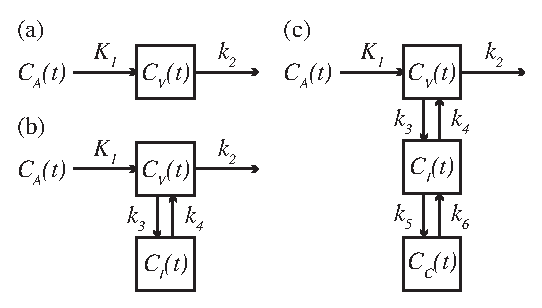
\includegraphics[width=\linewidth]{CompartmentalModels.eps}
    \end{minipage}
    \begin{minipage}{0.53\linewidth}
        \centering 
        \begin{tabular}{l} 
            \toprule
            $\frac{dC_{1}(t)}{dt} = K_{1} C_{0}(t) - k_{2} C_{1}(t)$ \hfill (a) \\ 
            \midrule
            $\frac{dC_{1}(t)}{dt} = K_{1} C_{0}(t) - (k_{2} + k_{3}) C_{1}(t) + k_{4} C_{2}(t)$ \\ 
            $\frac{dC_{2}(t)}{dt} = k_{3} C_{1}(t) - k_{4} C_{2}(t)$ \hfill (b) \\ 
            \midrule
            $\frac{dC_{1}(t)}{dt} = K_{1} C_{0}(t) - (k_{2} + k_{3}) C_{1}(t) + k_{4} C_{2}(t)$ \\ 
            $\frac{dC_{2}(t)}{dt} = k_{3} C_{1}(t) - (k_{4} + k_{5}) C_{2}(t) + k_{6} C_{3}(t)$ \\
            $\frac{dC_{3}(t)}{dt} = k_{5} C_{2}(t) - k_{6} C_{3}(t)$ \hfill (c) \\ 
            \bottomrule
        \end{tabular}
    \end{minipage}
    \caption{Block diagrams and first-order differential equations of compartmental models with (a)~one tissue compartment, (b)~two tissue compartments, (c)~three tissue compartments. $C_{0}(t)$ is the contrast-agent concentration in blood, $C_{1}(t)$ is the tissue intravascular concentration, $C_{2}(t)$ is the tissue interstitial concentration, $C_{3}(t)$ is the tissue intracellular concentration. $K_{1}$ is the unidirectional transfer rate of contrast-agent from blood to tissue vascular space, and $k_{2}$ is the unidirectional transfer rate of contrast-agent from the tissue vascular space to blood. Similarly $k_{3}$ and $k_{4}$ are the unidirectional transfer rates of contrast-agent between tissue vascular space and interstitial space, and $k_{5}$ and $k_{6}$ are the unidirectional transfer rates of contrast-agent between interstitial space and intracellular space.}
    \label{fig:compartmentalModels}
\end{figure}


% Kety:1944iv, The Quantitative Determination of Cerebral Blood Flow in Man by the Use of Nitrous Oxide in Low Concentrations
% Kety:1948je, The nitrous oxide method for the quantitative determination of cerebral blood flow in man: theory, procedure and normal values
Early use of compartmental models to fit indicator-dilution curves was based on the Fick\'s principle that relates the blood flow to the arterial and venous measurements~\cite{Kety:1944iv,Kety:1948je}.
In \citeyear{Kety:1944iv}, \citet{Kety:1944iv} derived a method to estimate cerebral blood flow from arterial and ven`ous blood sampling during inhalation of nitrous oxyde, and assessed it in a clinical experiment with eleven subjects.
The method corrected for the rise of the time-concentration curve using a fixed ratio of the amplitude of the monoexponential model fitted to the decay phase. 
% Kety:1951tp, The theory and applications of the exchange of inert gas at the lungs and tissues.
Following these developments, the authors proposed a one-compartment model based on the same principle to assess fractional blood flow and fractional blood volume assuming a perfectly diffusible tracer~\cite{Kety:1951tp}.

% Renkin:1959te, Transport of potassium-42 from blood to tissue in isolated mammalian skeletal muscles.
In \citeyear{Renkin:1959te}, \citet{Renkin:1959te} studied capillary permeability to $^{42}$K in skeletal muscles using another diffusion model based on Fick's law through in vivo radioactivity measurements of the arterial and venous blood.
The authors were among the first to use the permeability surface product as a combined parameter of the model, and established its correspondance to the maximum capillary clearance possible for a given substance assuming an infinite flow.
However they proposed a method to quantify the clearance at any flow rate assuming the permeability surface product is known.
They suggested that variations of the estimated permeability surface product were due to hemodynamic factors following either of the three following pattern: arteriovenous shunting, inhomogeneous flow distribution, or flow-dependant perfusion network.
They were however unable to determine which pattern was actually explaining the correlation between blood flow and permeability surface product in their data.

% Crone:1963cz, The Permeability of Capillaries in Various Organs as Determined by Use of the ‘Indicator Diffusion’ Method
In \citeyear{Crone:1963cz}, \citet{Crone:1963cz} developed the indicator diffusion method that relates the capillary permeability to blood flow, capillary surface area, and initial extraction which corresponds to the fractional reduction of the arterial concentration, however litterature values for the two first parameters were used and only the initial extraction was estimated.
The authors performed blood sampling experiments in dogs with injection of Evan's blue dye or a combination of inulin and sucrose to study the capillary permeability of these substances in multiple tissues, i.e.~brain, kidney, liver, lung, hind limb, by means of invasive catheterization.
Their study contradicts the results of \citet{Renkin:1959te}, and suggest that the discrepencies are due to a conceptual difference between the two studies regarding the definition of \``extraction\''.
But also because in the approach proposed by \citet{Renkin:1959te}, the presence of tracer outside capillaries was neglected despite the steady state reached by the system during the experiment.
Oppositely the approach proposed in this study relies on non-steady state measurements, ensuring lower extracapillary concentrations, and allowing accurate permeability estimates.

The theoretical developments presented in the three approaches above served as the foundation for compartmental analysis of perfusion exams.
The following sections present the adaptation of compartmental models to quantify perfusion in nuclear medicine, x-ray, magnetic resonance, and ultrasound imaging.
When comparing approaches, one should consider the characteristics of the tracer (intravascular vs.~diffusing, reversible vs.~irreversible), the characteristics of the vasculature in the tissue of interest (single vs.~dual input), the estimation method (linear vs.~non-linear).

\subsection{Nuclear medicine}

Many compartmental analysis developments in the field of nuclear medicine, and in particular positron emission tomoraphy (PET), were motivated by metabolic studies such as the consumption of glucose.
These metabolic measurements were permited by the development of labelled tracers, and in particular of labelled glucose.
Indeed, at the cellular level high consumption of glucose is synonym of fast metabolism.
Studying the consumption of glucose can reveal information on the cellular activity in the tissue, which is particularly relevant to study neuronal activity or to detect tumors and assess their malignancy.

% Gjedde:1981ge, High- and low-affinity transport of D-glucose from blood to brain
In \citeyear{Gjedde:1981ge}, \citet{Gjedde:1981ge} used a formula from \citet{Crone:1963cz}, and the previous developments of the group presented in~\cite{Gjedde:1980kh}, to derive two integral methods to estimate rate constants of glucose from blood to brain tissues in rats using scintigraphy measurements of blood sampled following the injection of a mixture of a $^{3}H$-labelled substance (D-glucose, L-glucose, D-mannitol, or sucrose), with $^{14}$C-butanol and $^{111}$InCl.
The methods consider the exchanges between the capillary and extracellular spaces, as well as the metabolic pools reflecting consumption of glucose by brain cells.
The first method estimated the initial rate constant as the difference of the total amount of tracer in the brain and the amount of plasma in brain twenty seconds after injection, normalized by the area under the arterial curve up to twenty seconds.
The second method exploited dynamic measurements to derive a graphical method, allowing the conjoint estimation of initial rate constant, and plasma volume, respectively as the slope, and intercept in the linear regression analysis of the ratio of the total amount of tracer in the brain to the arterial concentration, and the ratio of the total amount of tracer that passed in the artery to the arterial concentration.
Their experiments led them to the conclusion that the two methods estimated two different transfer rates, reflecting at least two transport mechanisms, i.e.~a high affinity system with low capacity, and a low affinity system with high capacity.

% Graphical methods for irreversible tracers
% Patlak:1983id, Graphical Evaluation of Blood-to-Brain Transfer Constants from Multiple-Time Uptake Data
Similarly, \citet{Patlak:1983id} proposed a graphical analysis method in \citeyear{Patlak:1983id} to estimate transfer constants across the blood-brain barrier for irreversible tracers.
The method is able to estimate the influx rate in any membrane system composed of at least one region with reversible exchanges without metabolisation where the tracer rapidly equilibrates with the plasma and one region with irreversible exchanges.
The methods consists in ploting the ratio of the curve in the tissue of interest to the plasmatic curve vs. the ratio of the integral of the plasmatic curve to the plasmatic curve, and fitting a affine model to the linear portion of the resulting curve that corresponds to the steady-state of the system.
The slope of the fitted linear model yields the influx rate from plasma to tissue, while the intercept yields an upper bound to the reversible plus plasmatic fractional volumes.

% Patlak:1985bc, Graphical evaluation of blood-to-brain transfer constants from multiple-time uptake data. Generalizations.
\citet{Patlak:1985bc} then generalized the method to analyze time-intensity curves using a reversible reference tissue instead of the arterial measurement, yielding an estimate of the ratio of the influx rate of the tissue to the sum of the reversible and plasmatic fractional volumes.
They also addressed cases when tracer binding is incomplete in the irreversible compartment, for both arterial and reference measurements, and presented specific applications of the method in the case of one reversible region (with or without re­versible binding) and one irreversible region.

% Graphical methods for reversible tracers
% Logan:1990jg, Graphical analysis of reversible radioligand binding from time-activity measurements applied to [N-11C-methyl]-(-)-cocaine PET studies in human subjects.
In \citeyear{Logan:1990jg}, \citet{Logan:1990jg} proposed a graphical analysis method to analyze the kinetics of reversible tracers, binding reversibly to receptors or enzyme, and applied it to estimate the parameters of the three-compartment model to characterize the binding of a radiolabeled cocaine complex in a PET study.
This is an extension of the method proposed by \citet{Gjedde:1981ge} to account for rapid binding and unbinding of the tracer where the graphical analysis is performed similarly.
Arterial blood was sampled throughout the experiment, and the arterial concentration in radiolabeled cocaine complex was used as an input of the model.
In terms of two-compartment model, the distribution volume can be derived from the slope of the linear portion of the plot.
In terms of three-compartment model, an additional measurement is necessary to determine the ratio of binding to unbinding rate from the ratio of the slopes in a receptor tissue to a non-receptor tissue assuming the plasmatic volume is negligible. 

% Logan:1996be, Distribution Volume Ratios Without Blood Sampling from Graphical Analysis of PET Data
The authors later extended the graphical analysis method to estimate distribution volume ratios~\cite{Logan:1996be}, defined as the ratio of the distribution volume of a tracer in a receptor tissue to a receptor-free tissue. 
The method allows the estimation of the distribution volume ratio from studies without arterial blood sampling, using only the curves extracted from the image in two regions. 
The direct distribution volume ratio estimation using the proposed method was compared to the ratio of the distribution volumes in the two tisues obtained using blood sampling data in a PET study with injection of $^{11}$C-labelled raclopride or d-threo-methylphenidate.
The method requires the knowledge of the average tissue to blood rate constant, as well as the determination of the initial time at which the slope should be estimated, which can be obtained from baseline experiments requiring blood sampling for calibration.

% Logan:2001ip, A strategy for removing the bias in the graphical analysis method.
In case of noisy data, this linear formulation of the compartmental modeling can yield underestimated distribution volume estimates because the errors are cumulative in the integral terms~\cite{Feng:1993cq}.
\citet{Logan:2001ip} proposed a strategy to remove the bias in the graphical analysis method, using the generalized linear least-squares algorithm proposed by \citet{Feng:1996ic} to determine the distribution volume directly for one-compartment models or as a smoothing technique prior to graphical analysis for more complex model structures.
The authors demonstrated the improved accuracy of the new estimation method, applied to evaluate either the distribution volume using an arterial input function, or the distribution volume ratio using a refrence tissue, in PET experiments following injection of $^{11}$C-labelled raclopride or d-threo-methylphenidate.
To estimate the distribution volume, an arterial input function was measured (for both tracers) from sampled blood.

% Non-linear formulation of compartmental models
% Hawkins:1984da, A kinetic evaluation of blood-brain barrier permeability in human brain tumors with [68Ga]EDTA and positron computed tomography.
In \citeyear{Hawkins:1984da}, \citet{Hawkins:1984da} used a two-compartment model based on the equation of the graphical analysis with a vascular component to evaluate the blood-brain barrier permeability in human brains using PET exams and $^{68}$Ga-EDTA as a tracer.
However they directly estimated the parameters of the model using a non-linear least-squares algorithm to fit the model, after resolution of the differential equations that relates the curve in the tissue of interest to the arterial blood sampling measurements.
The non-linear resolution of the equations yields a convolution formulation assuming a monoexponential decay in the tissue impulse reponse.
The method was used to estimate influx and outflux rate constants, as well as the blood volume fraction from which estimates of the regional cerebral blood volume corrected for the differences in hematocrit were derived, and compared it to direct estimation obtained using a three-compartment model previously described by~\citet{Phelps:1979tl}.

% Ziegler:1996cs, Measurement of liver blood flow using oxygen-15 labelled water and dynamic positron emission tomography: Limitations of model description
In \citeyear{Ziegler:1996cs}, \citet{Ziegler:1996cs} compared a dual-input and a single-input one-compartment model regarding their ability to quantify blood flow in dog liver using dynamic PET data following injection of a bolus of $^{15}$O-labelled water.
The dual-input model accounts for the arterial and portal supplies of the liver, using direct measurements resulting from blood sampling in the aorta and in the portal vein.
In the single-input model the determination of the portal supply is part of the fitting procedure, and is derived from the arterial measurement resulting from blood sampling by considering a gut compartment, based on a one-compartment model, which distribution volume was fixed and derived from post-mortem experiments in dogs.
Additionally the models correct for time-delays and dispersion using the method presented in~\cite{Meyer:1989vy}.
Both models make the assumption that the blood supplies diffuse instantaneously from vasculature to the liver tissue, and that the volume of distribution of the tracer is the same for arterial and portal blood.
For both models, the volume of distribution in the liver was not estimated but fixed for all experiments using the average value of the ratio of the arterial to liver concentrations in the late phase, assuming an equlibrium was reached.
The authors investigated the impact of this parameter on the estimation process, and reported a high sensitivity of liver blood flow, dispersion and fit accuracy to the fixed distribution volume value.
The single-input model additionally enforces a fixed ratio of gut tissue to liver tissue volume.
Poor agreement of the blood flow estimates of the dual-input and single-input models was found with microsphere measurements, however the single-input model performed slighlty better.

% Linear formulation of compartmental models
% Blomqvist:1984jy, On the Construction of Functional Maps in Positron Emission Tomography
In~\citeyear{Blomqvist:1984jy}, \citet{Blomqvist:1984jy} proposed a linear formulation of a three-compartment model, accounting for both metabolized and unmetabolized tracer, presented by~\citet{Raichle:1975va} obtained by rearranging and integrating twice the second-order differential equations relating the arterial concentration to the tissue concentration.
The method was used to derive functional maps from dynamic PET data of various tracers labelled with $^{11}$C, i.e.~$^{11}$C-methionine, $^{11}$C-deoxyglucose, $^{11}$C-glucose.
The authors did not report the method used to acces the arterial tracer concentration.
The three-compartment model was composed of a vascular compartment, and two extravascular compartments, one representing the extravascular space exchanging with the plasma, where the tracer is unmetabolized, and the other representing the metabolized compartment.
The authors estimated the tracer transfer rate constants from blood to tissue and from tissue to blood, as well as its metabolizing rate, by solving the system of equations using a linear least-squares methods.
The proposed linear estimation method was compared to the non-linear estimation of the three-compartment model, and good agreement were found between the estimates of the two methods, especially for blood to tissue transfer rate, and for the cerebral metabolic rate for glucose utilization, a composite index which definition can be found in~\cite{Reivich:1982ir}.

% Review papers
In \citeyear{Gunn:2001cx}, \citet{Gunn:2001cx} reviewed the compartmental models used for quantification of dynamic PET data, whether assessing perfusion, metabolism or ligand binding.
This theoretical study investigates both models using arterial input functions and models using reference tissues, as well as reversible and irreversible tracers, regardless of the number of compartments involved. 
General solutions for the impulse response are given in the form of sum of weighted exponential functions, which weight and rate constant have to be determined.
The authors differentiated micro parameters, i.e.~the actual rate constant parameterizing the model, from macro parameters, i.e.~global parameters defined as a function of the model rate constants, and showed that all the micro parameters of a perfusion model cannot be estimated individually, instead one should interpret the macro parameters in terms of the micro parameters, as the estimation of the latter was shown to be more stable.
Additionally, investigating models using a reference tissue region they showed that the macro parameters are expressed relatively to the reference region, and proposed a correction for the bias in graphical estimation methods when the contribution of blood in the reference and studied tissues cannot be neglected.

In \citeyear{Watabe:2006uy}, \citet{Watabe:2006uy} also proposed a review of compartmental models for quantification of dynamic PET data, especially addressing the models for the quantification of binding tracers.
The classical model counts four compartments, i.e.~an arterial compartment exchanging with a free compartment, that exchanges with a specific binding compartment, and a non-specific binding compartment.
The specific binding compartment is generally the compartment of interest when studying binding tracers.
If the non-specific binding compartment is in equilibrium with the free compartment, then these compartments can be merged, reducing the number of parameters by two.
Similarly, the simple one-compartment model, that only considers the exchanges between plasma and tissue through two rate constant parameters, can be used in flow limiting conditions, i.e.~when a quick equilibrium is reached between the free compartment and the binding compartment, or when using non-binding intravascular tracers.

\subsection{X-ray imaging}

% Yeung:1992wy, In vivo CT measurement of blood-brain transfer constant of iopamidol in human brain tumors.
In \citeyear{Yeung:1992wy}, \citet{Yeung:1992wy} used a two-compartement model to quantify the blood-to-brain impulse response of iopadimol, as well as plasmatic blood volume, using dynamic X-ray CT in a clinical study of brain tumors.
The two compartments correspond to the cerebral plasma space and the extravascular extracellular space, exchanging tracer with each other through the blood brain barrier assuming permeability limiting conditions.
The arterial measurements resulted from blood sampling measurements in a radial artery.
The clinical experiments revealed the ability of the estimated parameters to differentiate between healthy white and gray matter, tumor tissue, and metastatic tissue.
Indeed, higher values of both parameters were found in tumors and metastases.
Additionally, parametric maps of blood to brain impulse response and plasmatic blood volume were derived from the dynamic perfusion images, revealing the tumor functional heterogeneity.

% Graphical analysis
% Tsushima:1999ub, Functional CT of the kidney.
In \citeyear{Tsushima:1999ub}, \citet{Tsushima:1999ub} used a graphical analysis technique based on the work of \citet{Patlak:1983id} to estimate the fractional blood volume and the contrast clearance rate per unit volume of tissue (which is closely related to glomerular filtration), using perfusion X-ray CT of healthy (n = 82) and diabetic (n = 33) human kidneys following the intravenous injection of a bolus of iodinated contrast agent. 
The model uses an image-based arterial input function defined as the average enhancement curve in the manually segmented abdominal aorta region.
The authors reported a negative correlation of the patient age with the fractional clearance rate, but not with the fractional blood volume despite a tendency to decrease with age. 
A linear relation was found between X-ray CT estimates and the creatinine clearance rate obtained from urine sampling, which was the clinical reference method to estimate the glomerular filtration rate.

% Harvey:1999wa, Imaging of tumour therapy responses by dynamic CT.
In \citeyear{Harvey:1999wa}, \citet{Harvey:1999wa} used the same method to estimate the contrast clearance rate and the fractional blood volume of various tumor types in an attempt to assess tumor response to radiotherapy.
Acquisitions were performed before treatement for baseline, then early and late response exams were acquired one or two, and six to twelve weeks after treatement, respectively.
Authors showed an increase in the clearance rate as well as in the fractional blood volume in the early response exams, indicating an hyperemic response to radiotherapy.
Later exams revealed a decrease in parameter values compared to the early response, but still exhibited larger values when compared to the baseline experiments.

% Materne:2000gu, Non-invasive quantification of liver perfusion with dynamic computed tomography and a dual-input one-compartmental model.
In \citeyear{Materne:2000gu}, \citet{Materne:2000gu} used a dual-input compartmental model, similar to the model proposed by \citet{Ziegler:1996cs} for PET, to characterize liver perfusion from dynamic contrast-enhanced X-ray CT experiments accounting for both arterial and portal blood supplies.
The proposed method accounted for time-delays, but not for dispersion as originally proposed by \citet{Ziegler:1996cs}. 
The arterial and portal curves were extracted directly from the dynamic images, which was not possible with PET data due to the poor spatial resolution of the imaging modality.
Two models were actually considered, in the first one only the liver tissue component was considered, and in the second one the measured kinetics was considered a linear combination of the tissular, arterial, and portal components.
Hepatic, arterial, and portal perfusion indices were derived from the estimated model parameters.
The perfusion obtained with the first approach exhibited a strong correlation with microsphere measurements, which was not true for the second approach.
The reproducibility of the first approach was then investigated in a clinical experiment with healthy patients, and a good inter- and intra-observer agreement was reported.

\subsection{Magnetic resonance imaging}
% Tofts:1999ih, Estimating kinetic parameters from dynamic contrast-enhanced T(1)-weighted MRI of a diffusable tracer: standardized quantities and symbols
In \citeyear{Tofts:1999ih}, \citet{Tofts:1999ih} introduced compartmental models for the quantification of perfusion parameters using diffusible tracers in dynamic contrast-enhanced MRI, as well as a set of standardized notations for these parameters.
The authors adapted the methods developed for quantification of PET based on an arterial input function~\cite{Kety:1951tp,Renkin:1959te,Crone:1963cz} to MRI assuming the contribution of intravascular contrast-agent to signal intensity can be ignored.
They then derived a generalized model parameterized by the transfer constant from plasma to tissue noted $K_{trans}$, the extravascular extracellular space volume fraction noted $V_{e}$, and defined the rate constant as the ratio of these two parameters, noted $k_{ep}$.
The transfer constant is equivalent to the permeability surface area product under permeability-limited conditions, to blood flow under flow-limited conditions, and to extraction ratio under mixed conditions.
They also showed that the rate constant parameter is the decay rate of the exponential impulse response by solving the first-order differential equation of the generalized model.
This paper is much theoretical, however it assumes the arterial input function is estimated from the dynamic MR images, which measures whole blood contrast-agent concentration (as opposed to blood plasma) and shoud therefore be corrected for the hematocrit.
This paper became a standard in the field of perfusion imaging for MRI, for it introduced a set of clear and general notations that can be used to model the kinetics of any diffusible contrast agent.

% Murase:2004kr, Efficient method for calculating kinetic parameters using T1-weighted dynamic contrast-enhanced MRI
In \citeyear{Murase:2004kr}, \citet{Murase:2004kr} proposed a linear formulation of the generalized kinetics model presented by \citet{Tofts:1999ih}, additionally accounting for the vascular component of the signal. 
The main difference with the non-linear formulation originates in the resolution of the first-order differential equation, for which the author integrates both sides of the differential equation.
The tracer concentration in the tissue of interest is defined as the linear combination of the integral of the arterial measurement, the integral of the tissue measurement, and the arterial measurement itself, respectively weighted by the sum of the blood to tissue transfer constant with the product of the tissue to blood transfer constant with the volume fraction of blood in the tissue, the tissue to blood transfer constant, and the volume fraction of blood in the tissue.
The non-linear and linear resolution methods were compared through simulations in terms of accuracy and precision of the estimates, but also in terms of sensitivity to the sampling frequency.
The linear method was extensively faster, and more accurate in low to moderate noise conditions, and less sensitive to the sampling interval.
Additionally, the linear resolution method does not require initial values for the parameters, making the estimation method more robust.

% Balvay:2005ca, New criteria for assessing fit quality in dynamic contrast-enhancedT1-weighted MRI for perfusion and permeability imaging
In \citeyear{Balvay:2005ca}, \citet{Balvay:2005ca} investigated the sensitivity of two compartmental models for quantification of contrast-enhanced MRI to the duration of the acquisition using a new criteria to assess the quality of fit of the models in a preclinical study in mice with human prostatic tumors implantes subcutaneously.
A one-compartment model accounting for tissue perfusion only, and a two-compartment model accounting for both perfusion and permeability were fitted non-linearly to the mean enhancement curve in the tumor region using an image-based plasma measurement from the heart left ventricle.
The one-compartment model was not able to accurately fit the full-length mean enhancement curve in the tumor region and yielded biased tissue blood flow and fractional blood volume, but it was able to accurately fit shorter curves where permeability can be neglected and yielded parameter estimates comparable to those of the two-compartment model for full-length data.

% Kovar:1998bt, A new method for imaging perfusion and contrast extraction fraction: input functions derived from reference tissues.
In \citeyear{Kovar:1998bt}, \citet{Kovar:1998bt} faced limitations regarding the duration of their contrast-enhanced MRI acquisitions, and proposed a compartmental model using the contrast-agent kinetics in a reference tissue, such as a muscle, as well as litterature values of perfusion rate, extraction fraction, and extracellular volume in the chosen reference tissue to estimate the vascular input function.
This scheme was developed to reduce the high sampling frequency necessary to obtain a well resolved arterial input function, while avoiding invasive procedures, e.g.~blood sampling.
They then used the estimated input function to estimate the product of the perfusion rate and the extraction fraction in the tissue of interest.
The equations of the model were derived from the differential form of the model proposed by \citet{Kety:1951tp}.
The method was investigated in a preclinical magnetic resonance study of rats with implanted mammary and prostate tumors to assess the distribution of a diffusible paramagnetic tracer.

% Yankeelov:2005dea, Quantitative pharmacokinetic analysis of DCE-MRI data without an arterial input function: a reference region model.
Later, in \citeyear{Yankeelov:2005dea} \citet{Yankeelov:2005dea} proposed a method similar to that of \citet{Kovar:1998bt}, they however derived their equations from the integral form of the model proposed by \citet{Kety:1951tp} and used the standardized notations of \citet{Tofts:1999ih}. 
This formulation avoids the estimation of the arterial input function, and litterature values of the transfer constant from plasma to tissue and the distribution volume of the tracer in the reference tissue were used to directly derive estimates of these parameters in the tissue of interest.
The model was investigated through simulations to reveal the sensitivity of the model parameters to noise and to reference values.
The distribution volume parameter proved robust to noise using the proposed method, however the transfer constant from blood to tissue decreased with rising noise amplitude.
The authors also discussed the possibility to avoid the use of litterature values characterizing the reference tissue by defining relative parameters as the ratio of a parameter in the tissue of interest to its value in the reference tissue.

% Faranesh:2008tt, Incorporating a vascular term into a reference region model for the analysis of DCE-MRI data: a simulation study
In \citeyear{Faranesh:2008tt}, \citet{Faranesh:2008tt} proposed a modification of the model presented by \citet{Yankeelov:2005dea} to account for the intravascular tracer contribution to signal intensity in either or both of the studied and reference tissues.
Given litterature values of the vascular parameters characterizing the reference tissue, the arterial input function was estimated using two different formula depending on whether the vascular component was considered.
The estimated arterial input function was then used to estimate the perfusion parameters of the studied tissue assuming a two-compartment model, with or without a vascular compartment, and the linear formulation of the model introduced by \citet{Murase:2004kr}.
Simulations were conducted incorporating the vascular term, and the accuracy and precision of the parameters estimated using the modified reference region model were assessed using the model accounting for intravascular tracer in both the studied and reference tissues as a gold standard.
The simulations revealed that accounting for the vascular term in both the studied and reference tissues made the estimation exponentially dependent on the noise amplitude, although accounting for the fractional plasma volume in the studied tissue only yielded inaccurate estimation of all parameters.
The effect of the sampling frequency on the accuracy of the vascular parameter estimation revealed complex behavior.
The authors gave recommendations on whether the vascular term should be incorporated in the model depending on the information that can be found in the litterature about the expected range of vascular volumes in the studied and reference tissues, as well as on the ability of the sampling frequency to capture the vascular peak in the reference tissue kinetics.

% CardenasRodriguez:2013em, A linear algorithm of the reference region model for DCE-MRI is robust and relaxes requirements for temporal resolution
In \citeyear{CardenasRodriguez:2013em}, \citet{CardenasRodriguez:2013em} derived a linear formulation of the reference region model when the contribution of vascular tracer to signal intensity can be neglected in both the studied and reference tissues, as proposed by \citet{Yankeelov:2005dea}.
The linear formulation is obtained by integrating both sides of the equation derived by \citet{Yankeelov:2005dea} instead of solving it by part. 
The concentration of tracer in the tissue of interest is expressed as the linear combination of the tracer kinetics in the reference tissue, of its integral, and of the integral of the kinetics in the tissue of interest.
The weights of this linear model are respectively the relative blood to tissue transfer constant, the ratio of the transfer constant in the tissue of interest to the fractional distribution volume, and the rate constant in the tissue of interest.
These weights can therefore be estimated using a linear least-square fitting algorithm.
The authors compared the linear and non-linear estimation methods through simulation experiments, and studied the accuracy and the precision of the estimates, as well as the sensitivity of the parameters to the sampling frequency, the noise amplitude, the values of the parameters, and the shape of the arterial input function used to simulate the studied and reference kinetics.
Expectedly, in addition to alleviate the need for initialization values, the linear resolution method proved more accurate, especially for low sampling frequencies and high noise amplitudes.

\textbf{Kallehauge:2017ev, Comparison of linear and nonlinear implementation of the compartmental tissue uptake model for dynamic contrast-enhanced MRI.}

\subsection{Ultrasound}
To our knowledge, no proper compartmental approach had been proposed prior to the method proposed in \cite{Doury:2016fi} and in Chapter~\ref{chapter:IUS} of this document.
Indeed, compartmental models exhibit simple structures in contrast-enhanced ultrasound because the microbubbles remain strictly in the vascular bed, alleviating the need for additional extravascular compartments.

Recently, a compartmental model was used to characterize contrast-enhanced ultrasound data by \citet{Rizzo:2016dz}.
However the method is based on a gamma-variate model of the circulating bubbles with the addition of an irreversible compartment representing a fraction of microbubbles that can get trapped in complex vasculature.
This compartment is modeled by the addition of the integral of the fitted gamma-variate curve to the model, and the weight of this term must be estimated.
The model was fitted at the pixel level using a variational Bayes estimator which priors were derived from the non-linear fit of the same model at the regional level.
The authors reported a better fit in half of the pixel using the model with the irreversible compartment compared to a simple gamma-variate model in a cohort of 99 subjects suffering from arthritis.
They designed an automatic algorithm to detemine which model should be used according to the data.
The fraction of trapped microbubbles also improved classification of patients with rheumatoid and non-rheumatoid arthritis.


\section{Discussion}
From an experimental standpoint, the pioneering studies reviewed in this chapter suffer from major limitations which can be explained by the simultaneous development of the imaging technology, contrast agents, and quantification approaches.

Many of these studies used preliminary ultrasound contrast agents, known to be unstable and irregular in size, yielding poor resistance to injection and ultrasound pulses, as well as inconsistencies of the ultrasound signal.
All these characteristics made the quantification process of early studies extremely difficult.

Additionally, early contrast-enhanced imaging techniques were not contrast specific and exhibited low sensitivity, especially in the capillaries.
Moreover, contrast-enhanced ultrasound data was often acquired using a high mechanical index, causing the disruption of a large number of microbubbles.
Intermittent, or transient, imaging accounted for the disruptive nature of the high mechanical index but intrinsically forbit real-time perfusion imaging.
While microbubbles increased the sensitivity of Doppler techniques, allowing visualization of small and deep vessels, it fails to image the capillaries, and was generally of poor help to characterize moving structures.
Real-time non-destructive contrast-specific ultrasound imaging only arose with the development of pulse inversion sequences using low mechanical index in the late 1990s.

Most quantification approaches developed for contrast-enhanced ultrasound rely on indicator-dilution theory.
One of the main assumption underlying indicator-dilution theory is that the mass of the indicator is conserved throughout the experiment.
In vitro studies usually approximatively respect this condition when low mechanical index imaging is used, this is why these experiments are often extremely conclusive, and yield perfusion parameters in good agreement with the ground truth. 
However, in vivo, in addition to the natural and induced disruption, circulating microbubbles are partially filtrated through the lungs and liver, the mass conservation principle is therefore not respected.

Model-free quantification was common in early studies, it is however inherently sensitive to noise, especially as contrast-enhanced ultrasound time-intensity curves are corrupted by a multiplicative noise.
Therefore quantifying perfusion using parameters dependant on the peak-intensity is extremely unreliable, as it corresponds to the highest noise amplitude.
In pioneering cardiac studies, sampling frequencies were low and did not allow accurate characterization of the high-frequency wash-in resulting from bolus injection, therefore numerous studies focused on contrast-agent wash-out.

Following methodological and computational developements, model-based quantification was proposed to fit time-intensity curves, and allowed the estimation of many semi-quantitative parameters. 
While physical explanations were found for some explicit models, most studies merely used the models for noise filtering, correction of recirculation and time interpolation.
Indeed, semi-quantitative parameters were estimated from fitted curves, then blood flow and blood volume estimates were derived from indicator dilution theory.

Whether extracted directly from the time-intensity curve or from the modeled curve, semi-quantitative parameters are inherently sensitive to experimental conditions.
For instance, area under the curve, peak-intensity or even wash-in and wash-out rates, are directly related to the injected dose, moreover time parameters such as the wash-in and wash-out times, the time to peak-intensity or the mean transit time of the contrast agent are influenced by the site, speed and duration of the injection.

In addition, physiological parameters such as heart rate or even blood pressure can affect the kinetics or the ultrasound response of the microbubbles, and therefore affect the time-intensity curves. 
Because semi-quantitative parameters are directly extracted from the time-intensity curve, they suffer from physiological inter-exam variations too. 
This is also true for the replenishment of tissues following disruptive pulses in the case of infusion injection.

Because of the sensitivity of the semi-quantitative parameters to both experimental and physiological conditions, and because indicator-dilution theory is hardly applicable to contrast-enhanced ultrasound as discussed above, one should consider the derived parameters as relative indicators of perfusion, but certainly not as absolute parameters.

Deconvolution approaches estimate the response of a tissue to an instantaneous injection of tracer using an arterial input measurement, a tissue measurement, and none or little a priori on the shape of the estimated impulse tissue response.
Deconvolution methods based on the matrix formulation rely on matrix inversion, which is known to be an ill-conditioned problem.
Iterative algorithms were proposed to estimate the tissue impulse response without inverting the matrix, however they are extremely sensitive to noise as they are prone to cumulative error.
Unconstrained or poorly constrained deconvolution can sometimes yield impulse responses with negative values, which is not physiologically possible.
Constrained and regularized deconvolution were proposed to estimate positive, decreasing and smooth impulse response functions, but still few assumptions are made on the shape of the tissue response.

The shape of the estimated curves can be extremely heterogeneous depending on the estimation method and constrains, and extracting parameters can be difficult. 
To reduce the sensitivity of the deconvolution to noise and to limit oscillations of the tissue response, noise filtering techniques can be enforced rather simply in Fourier or singular value decomposition or by direct filtering of the time-intensity curve, but even small filtering errors can yield imprecise estimates.

Compartmental modeling roughly consist in a model-based deconvolution with strong a priori on the shape of the tissue impulse response and a reduced number of physiologically relevant parameters. 
The small number of degrees of freedom restricts the shape of the input function convolved with the tissue impulse respons to a limited set of possible curves, making the estimation process less sensitive to noise.
Linear formulations of these models can alleviate the need for initialization, but also make the estimation process more robust to noise, yielding stable estimates with fewer or sparser samples as discussed in Chapter~\ref{chapter:PLOSONE}.

An arterial measurement is required for some semi-quantitative approaches, by almost all deconvolution approaches, and by most compartmental models. 
Accurate arterial measurement allows the normalization of the tissue measurement and the estimation of perfusion parameters that are independant of the injection.

Arterial measurement can be performed through blood sampling, this technique is especially popular in the fields of nuclear medicine and radiology as continuous radioactivity measurements apparatus have been extensively developed and commercialized.
Nonetheless, patient needs to be catheterized and this procedure remains invasive. 

Image-based arterial measurements are extremely unreliable regardless of the imaging modality. 
Indeed the aorta is not always present in the field of view and a large artery feeding the tissue of interest can be hard to identify, especially in two-dimensional data.
Additionally, partial volume effect, attenuation and saturation artifacts can affect the measured signal intensity.
Indeed, in most modalities a trade-off must be made between space and time resolution, and the small size of the artery combined to the high speed of a bolus in an artery makes the estimation of the arterial input function extremely difficult.
In contrast-enhanced ultrasound the noise is multiplicative, which makes the high-intensity arterial measurements highly unreliable.

A healthy reference tissue can be chosen in the image to normalize the perfusion parameters in the tissue interest by their value in the reference region.
The reference region should be chosen in a large, homogeneous and well perfused tissue to limit partial volume effet and saturation artifacts in addition to reducing the noise in the reference tissue enhancement curve.

Direct estimation of relative perfusion parameters can also be obtained using compartmental modeling, alleviating the need for an arterial measurement.
The relative perfusion quantification methods were generally formulated with a single enhancement curve to characterize, even though they were often applied later to the region or even pixel level.

Whether fitting an explicit model to a single tissue curve for noise filtering or estimating quantitative parameters using a compartmental model using multiples enhancement curves, one should consider time-delay parameters.
Indeed, time-delay parameters are often overlooked in the litterature, however they play a crucial role in the estimation of perfusion parameters as fitting a model without a time-delay parameter or prior delay correction can induce a bias in the estimation.
A few methods were presented as delay-insensitive, some other methods actually include time-delay parameters in their equations, and commercial softwares certainly correct for delay, but to our knowledge no study reported on the absolute or relative values of such parameters, or exploited parametric maps revealing the timeline of the bolus arrival in the studied tissue. 
